%SPDX-License-Identifer: CC-BY-SA-4.0
%License-Filename: LICENSE

\documentclass[11pt,a4paper]{article}
\usepackage[T1]{fontenc}
\usepackage[utf8x]{inputenc}
\usepackage[ngerman]{babel}

\usepackage{geometry}
\geometry{	a4paper,
			top=25mm,
			left=25mm,
			right=25mm,
			bottom=20mm,
			headsep=4mm, 
			footskip=6mm
}
\usepackage{fancyhdr}
\usepackage{appendix}
\usepackage{float}
\usepackage{lastpage}
\usepackage{textcomp}

\usepackage{floatflt}
\usepackage{float}
\floatstyle{boxed}
\restylefloat{figure}


\usepackage{amsmath}
\usepackage{amsfonts}
\usepackage{amssymb}
\usepackage{units}

\usepackage{wrapfig}
\usepackage{graphicx}
\usepackage{xcolor}
\usepackage{hyperref}
\usepackage{courier}
\usepackage{lmodern}
\usepackage{url}

\usepackage{tikz}
\usetikzlibrary{positioning}
\usetikzlibrary{fit}

\usepackage{listings}
\lstset{ 
	backgroundcolor=\color{white},
	basicstyle=\footnotesize,
	breakatwhitespace=false,
	breaklines=true,
	captionpos=b,
	commentstyle=\color{green},
	extendedchars=true,
	frame=single,
	keepspaces=true, 
	keywordstyle=\color{blue},
	numbers=left,
	numbersep=5pt,
	numberstyle=\tiny\color{gray},
	rulecolor=\color{black},
	showspaces=false,
	showstringspaces=false,
	showtabs=false,
	stepnumber=1,
	stringstyle=\color{mymauve},
	tabsize=2
}

\usepackage{acronym}

\renewcommand\appendixtocname{Appendix}
\renewcommand{\headrulewidth}{0.4pt}
\renewcommand{\footrulewidth}{0.4pt}
\newcommand{\code}[1]{\textsf{#1}}
\newcommand{\pkg}[1]{\textsf{#1}}
\newcommand{\class}[1]{\textsf{#1}}
\newcommand{\printtitle}{Prototyp eines Multiinstanz-Managers für 
prozessvirtualisierte Anwendungen am Beispiel von OpenSlides}

\usepackage{tikz}

\title{\printtitle}
\author{Jochen Saalfeld}
\begin{document}
\nonfrenchspacing
\begin{titlepage}
	\begin{flushleft}
		\huge \printtitle
	\end{flushleft}
	\rule{\textwidth}{0.5pt}
	\large Bachelorarbeit von Jochen Saalfeld \\
	Universität Osnabrück
\end{titlepage}
\clearpage
\renewcommand\abstractname{Abstrakt}
\begin{abstract}
	Das Herkömmliche Applikationshosting entspricht den wachsenden 
	Anforderungen an dynamische Umgebungen immer weniger. Tools zur 
	Prozessvirtualisierung 	und Steuerung der Prozesse machen es Entwicklern, 
	Applikations- und Netzwerkarchitekten immer einfacher, ihre Applikationen 
	dynamisch zu provisionieren.\\
	\\
	Im Rahmen dieser Arbeit wird am Beispiel von OpenSlides 
	\url{https://openslides.org}, einem freien, webbasierten Software Tool für 
	die Verwaltung von Versammlungen, der Aufbau virtualisiert. Somit kann 
	OpenSlides dynamisch und flexibel für den Einsatz bei kleinen und großen 
	Veranstaltungen reagieren.\\
	\\
	Die bereits existierende Plattform zur Verwaltung mehrerer 
	OpenSlides-Instanzen wird evaluiert und an den aktuellen Stand der Technik 
	angepasst, um Kunden OpenSlides als \acf{SaaS} bereit zu stellen.
\end{abstract}
\renewcommand\abstractname{Abstract}
\begin{abstract}
	Traditional application hosting is becoming less and less responsive to the 
	growing demands of dynamic environments. Process virtualization and process 
	control tools make it increasingly easy for developers, application and 
	network architects to dynamically provision their applications.

	This work uses OpenSlides \url{https://openslides.org}, a free, web-based 
	software tool for the administration of meetings, as an example to 
	virtualize the structure and thus react dynamically and flexibly for use at 
	small and large events.

	The existing platform for managing multiple OpenSlides instances are 
	evaluated and updated to the current state of the art adapted to provide 
	customers with OpenSlides as \acf{SaaS}.
\end{abstract}
\clearpage
\tableofcontents
\clearpage
\pagestyle{fancy}
\fancyhead[L]{\rightmark}
\lfoot{\footnotesize{Seite \thepage~von \pageref{LastPage}}}
\cfoot{}
\rfoot{\footnotesize{Bachelorarbeit - Jochen Saalfeld}}
\parindent 0pt
\parskip 6pt
\section*{\printtitle}
Diese Arbeit wurde im Rahmen der Tätigkeit des Autors bei der Intevation 
GmbH\cite{inte} geschrieben. Der Autor des Dokuments ist seit über 2 Jahren bei
der Intevation GmbH angestellt und hat während seines Studiums dort gearbeitet. 
Die Intevation GmbH schreibt seit 1999 Freie Software, weswegen im Rahmen der 
Bachelorarbeit ausschließlich freie und/oder quelloffene Software betrachtet 
wird. Unter anderem hat der Autor an Gpg4win\cite{gpg4win} und 
OpenSlides\cite{oshp} mitgewirkt.

OpenSlides ist eine Django\cite{djangohp} basierte Web-Anwendung zur 
Unterstützung von Versammlungen. Mit der Software lassen sich mehrere 
Arbeitsabläufe abbilden, die bei der Verwaltung und Durchführung von 
Veranstaltungen unterstützen. OpenSlides bietet dabei unter anderem die 
Möglichkeit, Redelisten, Tagesordnungen, Anträge und Wahlen zu begleiten. 
Hierbei können alle Beteiligten an einer Veranstaltung auf die Software 
zugreifen und damit in verschiedenen Rollen interagieren\cite{oshp}. Intevation 
GmbH bietet auch Support und Hosting für OpenSlides bei Veranstaltungen 
an\cite{oscom}.

Beim herkömmlichen Applikationhosting von OpenSlides ist aufgefallen, dass bei 
Veranstaltungen mit vielen Teilnehmern entsprechend viel Kapazität beim 
Hosting der Applikation benötigt wird. Meist finden Veranstaltungen nur über 
einen beschränkten Zeitraum von wenigen Tagen statt. In diesen wenigen Tagen 
wird die gebotene Hardware gut genutzt; in den Wochen und Monaten der Vor- und 
Nachbereitung jedoch nicht. Hier wird die Möglichkeit gesehen, durch eine 
Prozessvirtualisierung der Software die Leistung besser zu nutzen, um so das 
Angebot für den Kunden attraktiver zu gestalten und den Fußabdruck der nötigen 
Ressourcen zu verkleinern.

Zuerst wird in Kapitel \ref{sec:pum} das Problem beschrieben und die Motivation 
erläutert. Daran anschließend wird es in Kapitel \ref{sec:einf} eine Einführung 
in das Thema geben. In Kapitel \ref{sec:sdt} der Stand der Technik 
erläutert. Anschließend wird in Kapitel \ref{sec:tun} die Technologiewahl 
erörtert und die Neuentwicklung beschrieben. In Kapitel \ref{sec:umsos} werden 
die Umsetzungen an OpenSlides beschrieben. Das darauf folgende Kapitel 
\ref{sec:umm} erläutert die Umsetzungen im Multiinstance-Manager. Abschließend 
gibt es im Kapitel \ref{sec:za} eine Zusammenfassung und einen Ausblick.
\clearpage
\section{Problembeschreibung und Motivation}
\label{sec:pum}
Schon früh ist bei der Bearbeitung von Hosting-Anfragen bei der Intevation GmbH 
für \mbox{OpenSlides} aufgefallen, dass vor allem unter Berücksichtigung des 
nötigen Datenschutzes, bei schützenswerten Informationen\cite{persBezDat} der 
Hardwareaufwand recht hoch ist. Durch die besonderen Eigenschaften und Auflagen,
die ein Rechenzentrum erfüllen muss, sind die Kosten deutlich höher. Eingangs 
wurde jede Instanz von OpenSlides auf einer eigenen Hardware zur Verfügung 
gestellt, damit Inhalte unter keinen Umständen in fremde Hände geraten können.

Die Konfiguration \glqq{}1 Instanz $=$ 1 Server\grqq{} bietet den höchsten 
Datenschutz, da jeder Mandant seine eigene Hardware hat und somit durch keine 
Fehler auf Daten anderer Mandanten bzw. Instanzen zugreifen kann. Jedoch ist 
diese Konfiguration auch die teuerste und ineffizienteste. Sie ist ineffizient, 
da bei Veranstaltungen die Leistung des Servers nur im Veranstaltungszeitraum 
selbst stark beansprucht wird. In der Vor- und Nachbereitungszeit wird hingegen 
nur ein Bruchteil der Leistung benötigt. Es wurde festgestellt, dass in dieser 
Phase weniger als $\frac{1}{10}$ der Nutzer in dieser Zeit OpenSlides 
verwenden. Diese Konfiguration ist zudem auch für den Kunden die teuerste 
Möglichkeit, OpenSlides einzusetzen, da er für den gesamten Einsatzzeitraum für 
einen Server bezahlen muss, von dem er über die meiste Zeit nur einen Bruchteil 
nutzt.

Die Motivation, den Kunden ein günstigeres Produkt anzubieten, muss jedoch 
weiterhin mit strengen Datenschutzrichtlinien einhergehen. Die Lösung für das 
Problem muss also in jeder Hinsicht der Konfiguration \glqq{}1 Instanz $=$ 1 
Server\grqq{} entsprechen.

Der direkte Weg, um dies zu erreichen, ist die Prozessvirtualisierung 
(\ref{subsec:sdtpv}) und Steuerung (Orchestrierung (\ref{subsec:sdtorch})) der 
virtualisierten Prozesse. Damit lässt sich eine Konfiguration von \glqq{}m 
Instanzen $=$ n Server\grqq{} erreichen.
\newpage
\section{Einführung}
\label{sec:einf}
Im vorherigen Kapitel \ref{sec:pum} wurde bereits kurz die Problematik 
umschrieben. In den folgenden Kapitel (\ref{subsec:introfo}) wird zunächst die 
funktionale (\ref{subsubsec:introfofb}) und anschließend die technische 
(\ref{subsubsec:introfotb}) Seite von OpenSlides beschrieben.

Zunächst werden im Unterkapitel \ref{subsec:introfo} die Funktionen von 
OpenSlides beschrieben. Dann werden in Kapitel \ref{subsec:introfomb} die 
Funktionen den OpenSlides-Multiinstance-Backends beschrieben, anschließend 
daran werden in Kapitel \ref{subsec:intropomb} die Probleme an diesem 
beschrieben. In Kapitel \ref{subsec:introloe} wird die Lösung der Probleme 
besprochen.
\subsection{Beschreibung von OpenSlides}
\label{subsec:introfo}
OpenSlides wird von verschiedensten Verbänden und Vereinen eingesetzt, um 
Veranstaltungen zu begleiten und den Ablauf zu digitalisieren. In Abbildung 
\ref{fig:osdemohome} wird die Seite dargestellt, die ein Nutzer zuerst sieht.
\begin{figure}[htp]
	\centering
	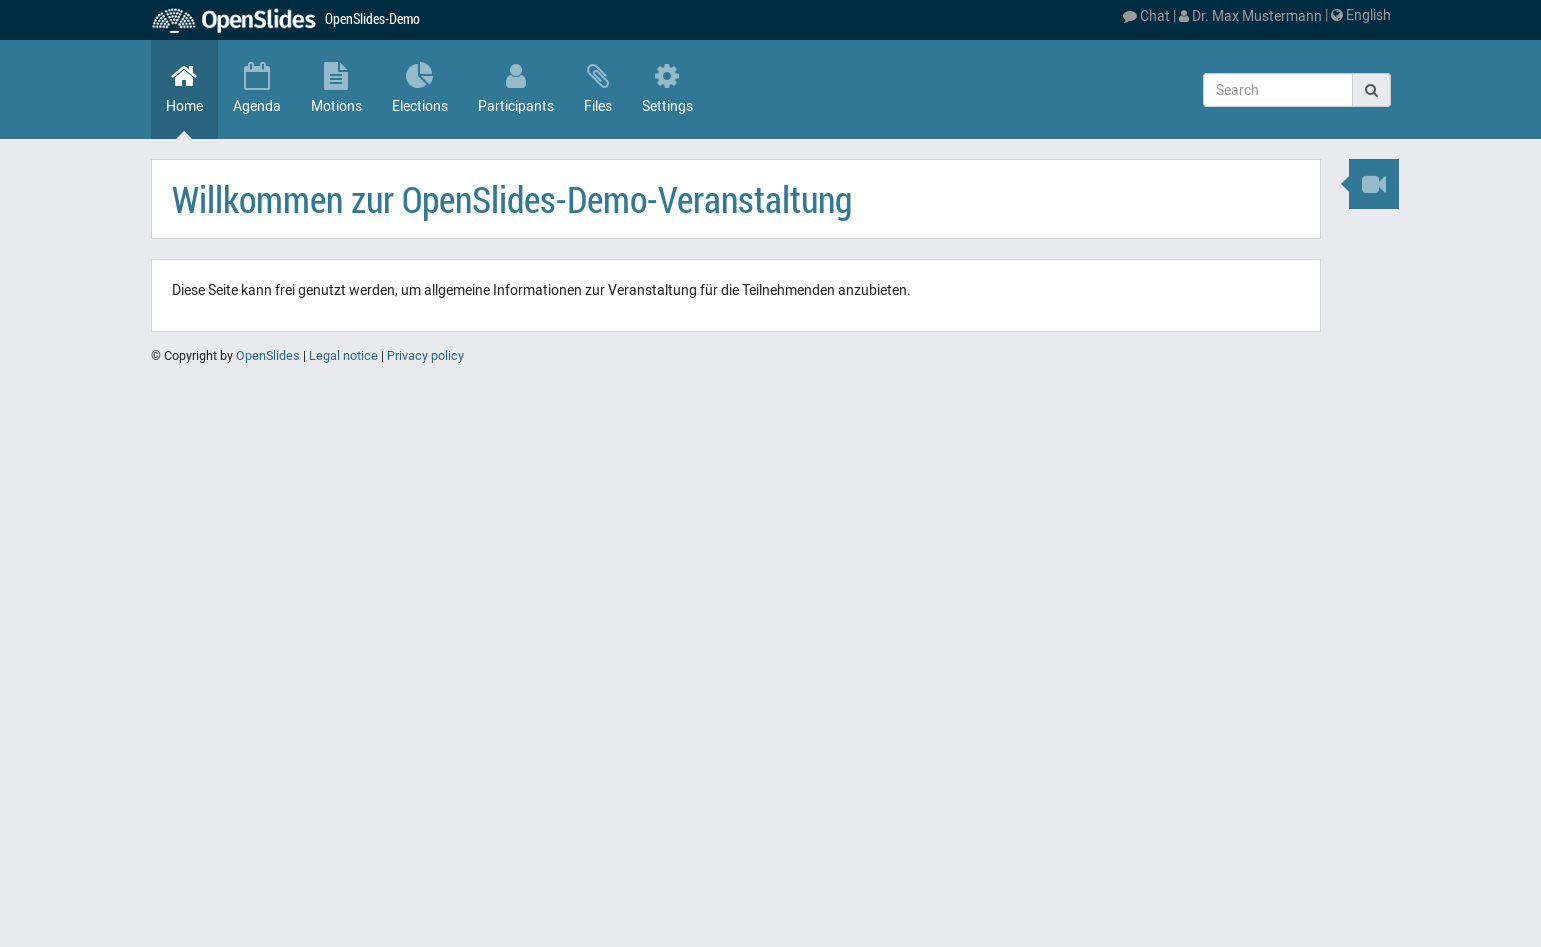
\includegraphics[width=0.95\textwidth]{img/openslides_home_page.png}
	\caption[OpenSlides-Demo-Instanz \glqq{}Home\grqq{}-Seite
	\cite{osdemo}]{OpenSlides-Demo-Instanz \glqq{}Home\grqq{}-Seite 
		\cite{osdemo}}
	\label{fig:osdemohome}
\end{figure}
\newpage
Die Übersicht in Abbildung \ref{fig:osdemoagenda} ist eine Tagesordnung einer 
Veranstaltung. Diese kann auch zur Projektion verwendet werden und führt die 
Nutzer durch die Veranstaltung.
\begin{figure}[htp]
	\centering
	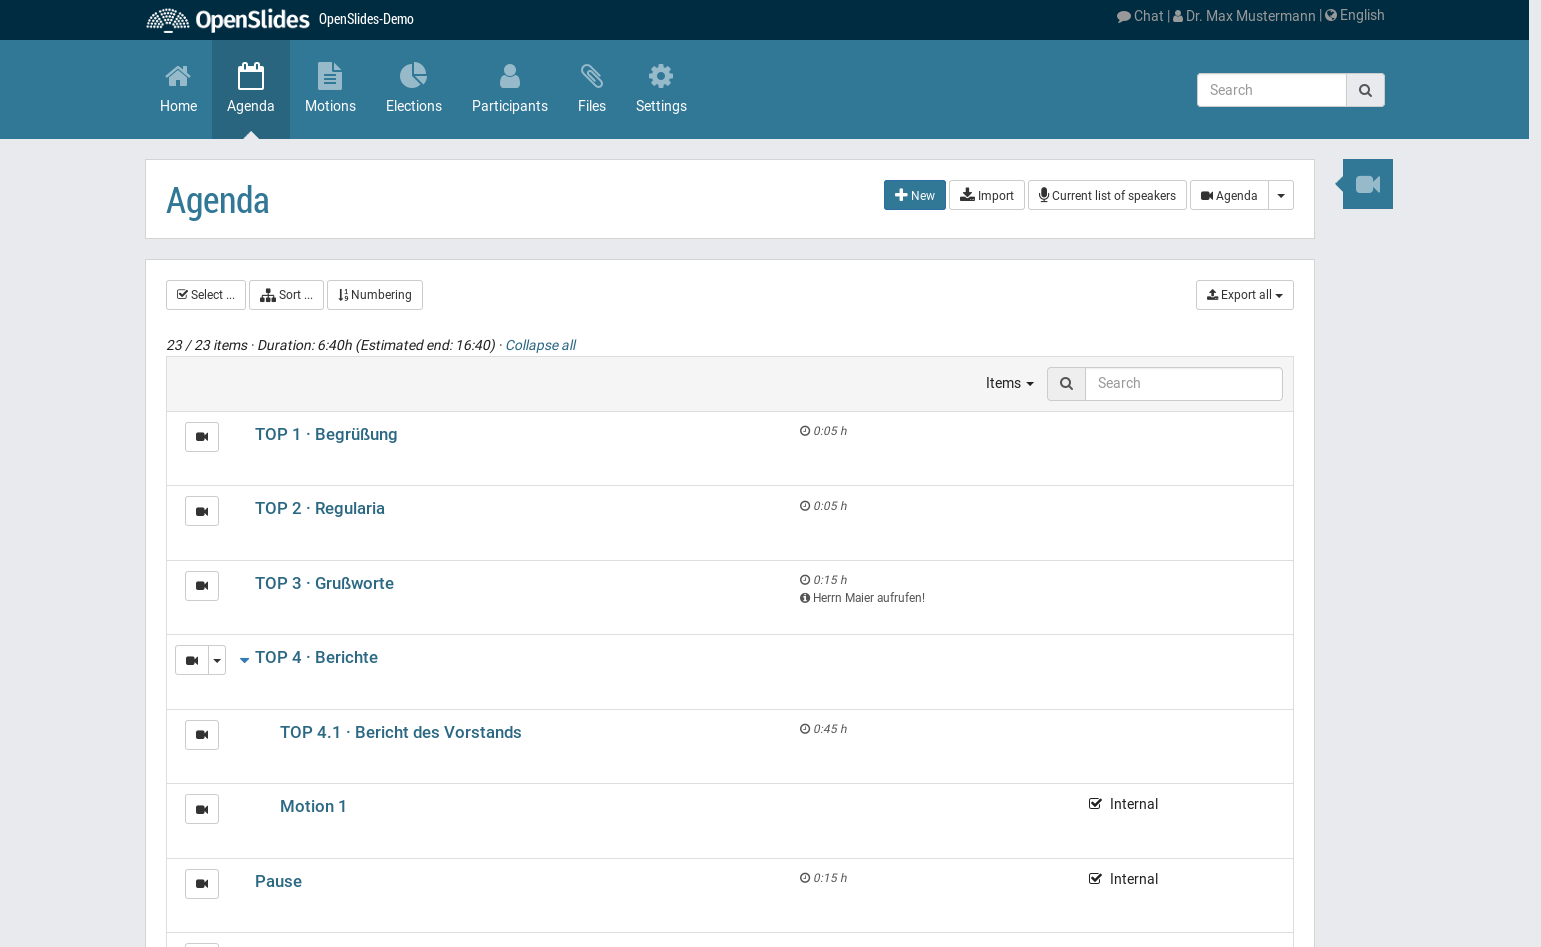
\includegraphics[width=0.87\textwidth]{img/openslides_agenda_page.png}
	\caption[OpenSlides-Demo-Instanz \glqq{}Agenda\grqq{}-Seite
	\cite{osdemo}]{OpenSlides-Demo-Instanz \glqq{}Agenda\grqq{}-Seite 
		\cite{osdemo}}
	\label{fig:osdemoagenda}
\end{figure}

Abbildung \ref{fig:osdemomotion} zeigt eine beispielhafte Antragsübersicht. 
Diese bietet den Nutzern die Möglichkeit, eine Übersicht zu erhalten und auf 
einem Blick den Status der Anträge einzusehen.
\begin{figure}[htp]
	\centering
	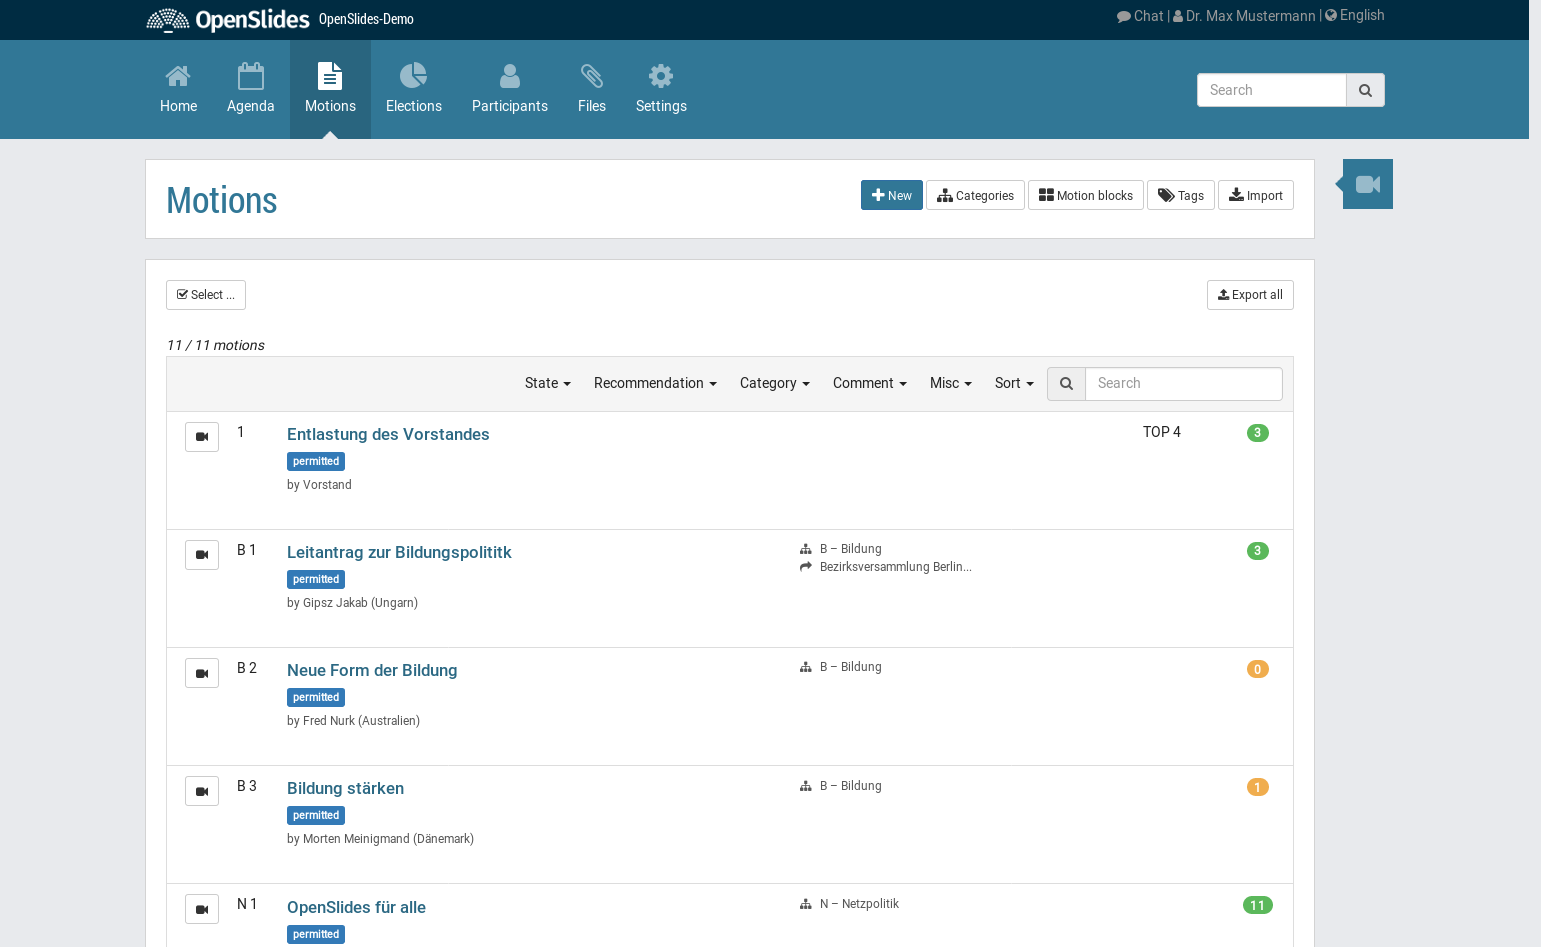
\includegraphics[width=0.87\textwidth]{img/openslides_motions_page.png}
	\caption[OpenSlides-Demo-Instanz \glqq{}Anträge\grqq{}-Seite
	\cite{osdemo}]{OpenSlides-Demo-Instanz \glqq{}Anträge\grqq{}-Seite 
		\cite{osdemo}}
	\label{fig:osdemomotion}
\end{figure}
\newpage
\subsubsection{Funktionale Beschreibung}
\label{subsubsec:introfofb}
OpenSlides \cite{oshp} ist eine Software zur Begleitung von Veranstaltungen, 
wie Mitgliederversammlungen. Sie unterstützt dabei die Organisation und 
Durchführung in folgenden Punkten:
\begin{itemize}
	\item Teilnehmerverwaltung
	\item Antragsverwaltung und -beratung (vgl. Abbildung 
		\ref{fig:osdemomotion})
	\item Tagesordnung (vgl. Abbildung \ref{fig:osdemoagenda})
	\item Anwesenheitskontrolle
	\item Durchführung und Auswertung von Wahlen
	\item Projektion
	\item Redelisten
\end{itemize}
Bei der Struktur und Mitglieder-Abbildung haben Organisationen die Möglichkeit, 
ihre Mitglieder in Gruppen zuzuordnen, sodass sie den Organisationsstrukturen 
in der Organisation selbst entspricht. Es können auch zusätzliche 
Gruppenzuordnungen gemacht werden, um die Adminstratoren der OpenSlides Instanz 
oder einzelner Funktionen festzulegen.

In der Antragsverwaltung oder Antragsberatung können verschiedene Arbeitsabläufe
genutzt werden, um den Abläufen der Organisationen gerecht zu werden. Aufgrund 
der verschiedenen Arbeitsflüsse und Einstellungen kann hier eingestellt 
werden, welche Mitgliedergruppen auf welche Funktionen Zugriff haben.

Die Tagesordnung kann, wie bei Versammlungen üblich, nach Tagesordnungspunkten 
sortiert werden. Einzelne Tagesordnungspunkte können auch Unterpunkte 
enthalten. Sie sind für alle Mitglieder einsehbar.

Durch die Anwesenheitskontrolle kann man markieren, welche 
Mitglieder tatsächlich einer Versammlung beiwohnen. Dies kann z.B. bei 
der Auswertung und Begleitung von Wahlen genutzt werden, um zu prüfen, ob alle 
Anwesenden oder mehr als die anwesenden Personen gewählt haben. Die Auswertung 
und Durchführung von Wahlen ist derzeit, ohne Plugins (wie z.B. dem OpenSlides 
Votecollector Plugin \cite{osvc}), nur analog möglich. Hierbei werden die 
Ergebnisse dann in OpenSlides eingetragen und können anschließend projiziert 
werden.

Dank der Projektion können Tagesordnungpunkte, Redelisten, Anträge und Wahlen 
über einen oder mehrere Beamer projiziert werden. Somit kann an einer Stelle 
die Versammlung geführt und geleitet werden.
\newpage
\subsubsection{Technische Beschreibung}
\label{subsubsec:introfotb}
Die OpenSlides-Architektur \cite{osgh} kann in verschiedene Pakete herunter 
gebrochen werden:
\begin{itemize}
	\item Kern %core
	\item Web-Darstellung %daphne
	\item Datenbank %postgres
	\item Zwischenspeicher %redis
	\item Anfragenverarbeitung %worker 
	\item Webserver %nginx
	\item Mail-Versender %postfix
\end{itemize}
Der Kern baut OpenSlides und richtet die einzelnen Komponenten ein. Er wird in 
der Regel nur einmal gestartet, kann aber auch zum Upgrade auf neuere 
Versionen erneut gestartet werden und übernimmt dabei die Migration.

OpenSlides basiert auf Django \cite{djangohp} im Backend und auf AngularJS 
\cite{angularhp} im Frontend. Die im Hintergrund von der Anfragenverarbeitung 
(sog. \texttt{worker} \cite{daphne}) generierten und ausgewerteten Inhalte 
werden zur Darstellung (\texttt{daphne} \cite{daphne}) zum Webserver 
(\texttt{nginx} \cite{nginx}) weitergeleitet.

Damit der \texttt{worker} die Anfragen auswerten kann, liest er sie aus dem 
Zwischenspeicher (\texttt{redis} \cite{redis}) und der Datenbank 
(\texttt{postgres} \cite{postgres}) aus. Um Nutzern Informationen, wie 
Passwörter oder Rundschreiben aus OpenSlides zukommen zu lassen, ist auch ein 
Mail-Versender (\texttt{postfix} \cite{postfixhp}) Teil des Gesamtsystems.

\begin{figure}[htp]
	\centering
	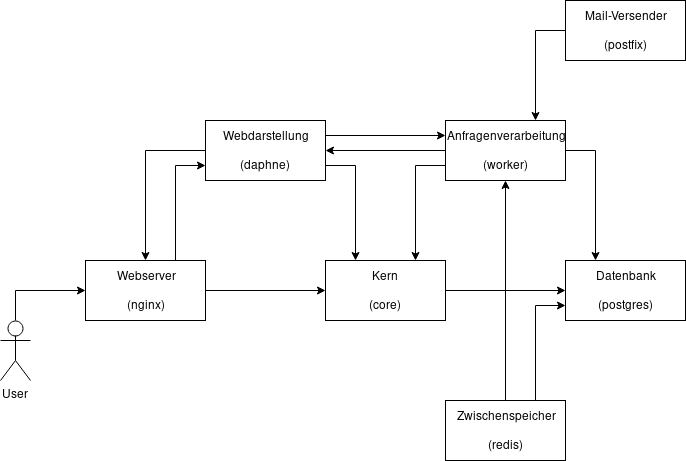
\includegraphics[width=0.87\textwidth]{img/techn_besch.png}
	\caption[OpenSlides - Technischer Aufbau]{OpenSlides - Technischer Aufbau}
	\label{fig:ostechbesch}
\end{figure}

In Abbildung \ref{fig:ostechbesch} kann man sehen, wie die Instanz aufgebaut 
ist, und welche Komponenten miteinander kommunizieren bzw. wie der Fluss der 
Daten unter den Komponenten ist.
\newpage
\subsection{Funktionsbeschreibung OpenSlides-Multiinstance-Backend} 
\label{subsec:introfomb}
Das OpenSlides-Multiinstance-Backend \cite{osmib} vereint alle Teile in der 
technischen Beschreibung \ref{subsubsec:introfotb}, bis auf die 
Datenbank auf einem \texttt{rkt} \cite{rkthp} basierenden Container. Die 
Container werden via \texttt{ansible} \cite{ansible} gestartet, gesteuert und 
konfiguriert. Die Verwaltung kann über einen Einzelnutzer in einer 
Weboberfläche gesteuert werden.

Die Datenbanken werden für alle Instanzen zentral auf dem Server verwaltet, wobei 
sie sich die Software-Instanz der Datenbank-Applikation teilen. Jede Instanz 
erhält dabei eine eigene Datenbank mit eigenem User in dem Cluster der 
Datenenbank-Software. Die Software an sich ist jedoch nicht pro Instanz 
getrennt.
\subsection{Problematik an OpenSlides-Multiinstance-Backend} 
\label{subsec:intropomb}
Eines der größten Probleme des in Kapitel \ref{subsec:introfomb} beschriebenen 
Multiinstance-Backends ist die geteilte Datenbank. In Kapitel 
\ref{subsubsec:introfotb} wurde beschrieben, dass unter anderem Personendaten 
und personenbezogene Daten in der Datenbank gespeichert werden. Dadurch, dass 
sich alle Instanzen die Datenbank auf dem Host-Betriebssystem teilen, kann es 
potentiell zu einem unerlaubten Zugriff kommen. Die geteilte Datenhaltung macht 
es auch nicht möglich, dass wir mehrere Mandaten in dem Multiinstanz-System 
halten.

Des Weiteren sind die Container, in denen die Instanzen laufen, nicht an ein 
Überwachungssystem angeschlossen. Somit können Probleme und Fehler, die zur 
Laufzeit auftreten, nicht zentral ausgewertet werden.

Da die ganze Instanz immer nur in einem Container läuft, kann sie auch nicht 
dynamisch auf größere Anfragen reagieren. Wenn die einzelnen Komponenten 
ausgelastet sind, können sie nur durch manuellen Eingriff skaliert werden. 
Diese Konfiguration eignet sich nicht für einen dynamischen Aufbau.
\subsection{Zielsetzung}
\label{subsec:introloe}
Die eingesetzten Technologien im Multiinstance-Backend (\ref{subsec:introfomb}) 
sollen auch weiterhin zum Einsatz kommen. Somit soll weiterhin 
Prozessvirtualisierung eingesetzt werden, um eine \glqq{}$n$ Instanzen = $1$ 
Server\grqq{} zu erreichen. Darauf aufbauend sollen Orchestrierung und 
Steuerung genutzt werden, um die virtualisierten Prozesse zu verwalten und eine 
\glqq{}$n$ Instanzen = $m$ Server\grqq{} Konfiguration zu erreichen. Dabei 
sollte vor allem die geteilte Datenbank eliminiert werden, damit das System 
mandantenfähig wird. Dies bedeutet, dass mehrere unterschiedliche Kunden über 
ein System verwaltet werden und, dass sie sich die Hardware teilen können. Des 
Weiteren sollen die Log-Einträge der einzelnen Instanzen zentral geführt werden,
und es soll eine einfache Möglichkeit geben, die Instanzen dynamisch auf 
Nutzeranfragen skalieren können.

Das Ziel soll sein, zu prüfen, wie das jetzige Multiinstance-Backend ersetzt 
werden kann. Dabei sollen die Kosten für den Kunden durch die Nutzung der 
gleichen Hardware und die Teilung des Systems so günstig wie möglich gehalten 
werden.
\clearpage
\section{Stand der Technik}
\label{sec:sdt}
Um einen Überblick zu gewinnen, welche Technologien verwendet werden können, 
werden alle marktüblichen Technologien betrachtet.

In Kapitel \ref{subsec:sdtpv} wird zunächst die Prozessvirtualisierung 
erörtert. Im darauf folgenden Kapitel \ref{subsec:sdtorch} wird die 
Orchestrierung dieser diskutiert.
\subsection{Prozessvirtualisierung}
\label{subsec:sdtpv}
Die Virtualisierung, die Nutzung von Software und Prozessen, als auch die 
Ausgliederung von Abhängigkeitsmanagement in Container, ist nicht erst ein 
Thema der letzten Jahre. Bereits 1979, als Unix in der Version 7 entwickelt 
wurde, konnte \texttt{chroot} eingeführt werden. Es bietet sich als 
Visualisierung nicht für OpenSlides an, da chroot keine Root Privilegien 
Isolation unterstützt.\cite{containerhist}

Zwischen 1972 und heute sind viele neue Tools hinzugekommen, die in 
irgendeiner Art und Weise die Virtualisierung von Prozessen unterstützen 
\cite{containerhist}. Es sollen jedoch nur jene betrachtet werden, welche die 
Spezifikationen der \acf{OCI}\cite{oci} unterstützen. Die \ac{OCI} hat sich im 
Jahre 2015 aus verschiedenen führenden Technologieanbietern im Bereich der 
Container basierten Virtualisierung gegründet, um einen offenen Standard zu 
entwickeln. Dieser wird von den Technologieführern\cite{ocimembers} entwickelt 
und implementiert. Im Rahmen der Betrachtung der Technolgien zur 
Prozessvirtualisierung werden nur Tools betrachtet, welche diesem Standard 
folgen. Diese Entscheidung wurde getroffen, da abzusehen ist, dass dieser 
Standard noch lange existiert und das auch über verschiedene Tools hinweg. Eine 
Zukunft ist also gesichert.

Durch den Standard, der durch die \ac{OCI} gepflegt wird, unterscheiden sich 
die Produkte nur noch in einigen Punkten. So kann lediglich die 
Beschreibungssprache zum Bereitstellen eines Containers als Image 
unterschiedlich sein.  Einmal erstellt, sind die Images durch jedes Tool 
nutzbar. Dann können die Images wiederum unterschiedlich durch die Werkzeuge 
behandelt werden. Den \glqq{}Rohling\grqq{} für einen Container nennt man 
Image.

Zur Zeit gibt es drei große Lösungen, welche den Richtlinien der \ac{OCI} 
folgen. Zum einen \texttt{rkt} (rock-it gesprochen), welches von den 
Entwicklern des Betriebssystems \grqq{}CoreOS\glqq{} im Jahre 2014 
veröffentlicht wurde\cite{rkthp}. Des Weiteren gibt es seit Kurzem 
\texttt{railcar} von \grqq{}Oracle\glqq{}, welches eine auf der 
Programmiersprache \texttt{rust} basierende Implementation des \ac{OCI} 
Standards ist\cite{railcarhp}. Weiter gibt es \texttt{docker} von der 
\glqq{}Docker Inc.\grqq{}. Sie sind Initiator der \ac{OCI}, mit der 
Veröffentlichung im Jahre 2013 seit längster Zeit auf dem Markt und mit über 13 
Milliarden Downloads (2017) Marktführer in dem Segment\cite{dockerdl}.
\subsection{Orchestrierung} \label{subsec:sdtorch}
Da die Anwendung skalieren soll, wird ein Werkzeug benötigt, mit dem die Anzahl 
der Container für die einzelnen Komponenten der Applikation angepasst werden 
können. Dabei wurde die Applikation in 4 Images unterteilet. Zunächst wird ein 
\texttt{nginx}\cite{nginx} Container als \glqq{}Proxy\grqq{} benötigt, um die 
Anwendung aus dem Web über die Standard-Ports erreichbar zu machen. Dahinter 
liegt \texttt{daphne}\cite{daphne}. \texttt{daphne} ist ein HTTP-basierter 
WebSocket-Protokoll-Server, der über die Channel-Technolgie aus Django die 
\texttt{worker}-Endpunkte anspricht, die wiederum jeweils ein Container sind. 
Schlussendlich gibt es noch \texttt{redis}\cite{redis} als Container, der für 
den Server-seitigen Cache bei den \texttt{worker}n sorgt und 
\texttt{postgres}\cite{postgres} im Container als Datenbank.

\texttt{redis} mit dem Cache und \texttt{postgres} mit den Daten ebenso wie der 
Proxy und Load Balancer \texttt{nginx} sind schlecht zu skalieren. Diese 
Container dürfen also nur einmal pro Instanz der Applikation gestartet werden. 
In der Dokumentation zu Openslides\cite{osgh} findet man das Beispiel, dass pro 
\texttt{daphne}-Instanz vier \texttt{worker} gestartet werden. Diese 
beiden Container können also im Verhältnis $1:4$ skaliert werden. Das Trennen 
der Instanzen in mehrere virtueller Netze und das Skalieren basiert auf 
Metriken (wie z.B. CPU-Auslastung oder Anzahl aktiver Nutzer) oder auf 
\glqq{}Knopfdruck\grqq{}, nennt man Orchesteriren.

Die in Kapitel \ref{subsec:sdtpv} genannten Tools bringen teilweise ihre 
eigenen Werkzeuge zur Orchestrierung mit, so bringt \texttt{docker} die 
Engine \texttt{docker swarm}\cite{dockSwarm} mit. Dieses arbeitet nativ mit 
\texttt{docker} und der Docker-Engine zusammen. Zusätzlich gibt es 
\texttt{kubernetes}\cite{kubernetes}, welches ursprünglich von Google 
entwickelt wurde, mittlerweile aber in Cloud Native Computing Foundation 
übernommen wurde. \texttt{kubernetes} vereinfacht das Verteilen von 
\texttt{containern} und bringt, wie \texttt{ansible}\cite{ansible} 
oder \texttt{puppet}\cite{puppet}, ähnliche Eigenschaften mit. Alle drei bieten 
Möglichkeiten zur automatischen Softwarebereitstellung, dem 
Konfigurations-Management und dem Applikations-Deployment; lassen sich aber 
auch für die Orchestrierung von Containern (teilweise mit Plugins) einsetzen. 
\texttt{kubernetes} und \texttt{docker swarm} sind von den genannten Tools die, 
welche eine gute Integration mit \texttt{docker} bieten.
\clearpage
\section{Technologiewahl \& Neuentwicklung} \label{sec:tun}
Durch die Spezifikationen des \ac{OCI} sind viele der Technolgien untereinander 
kompatibel, weswegen die Wahl für ein Tool zur Prozessvirtualisierung 
größtenteils unabhängig von der Wahl für ein Tool zur Orchestrierung 
stattfinden kann. Lediglich das Orchestrierungstool Docker Swarm ist von dem 
Prozessvirtualisierungstool Docker abhängig.

Zunächst wird in Kapitel \ref{subsec:tunpv} die Prozessvirtualisierung 
besprochen. Anschließend wird in Kapitel \ref{subsec:tunorch} die 
Orchestrierung dieser erörtert. Abschließend wird in Kapitel \ref{subsec:tunsu} 
auf den Server und die Umgebung eingegangen.
\subsection{Prozessvirtualisierung} \label{subsec:tunpv}
Wie in Kapitel \ref{subsec:sdtpv} erwähnt, unterscheiden sich die Werkzeuge 
\texttt{rkt}, \texttt{railcar} und \texttt{docker} nur in der 
Beschreibung der Images und in der Ausführung dieser. Wenn das Image dann 
bereit gestellt ist, sind sie untereinander kompatibel, können aber als 
breitgestellte Container wiederum unterschiedlich behandelt werden. Da 
\texttt{docker} der de-facto Industriestandard ist, werden die anderen 
Technolgien damit verglichen.

Bei einem Vergleich zwischen \texttt{docker} und \texttt{rkt} fallen nur wenige 
Unterschiede auf. Einer der bestechenden Unterschiede ist jedoch, dass 
Container, die mit \texttt{rkt} gestartet werden, mit Root-Rechten gestartet 
werden müssen. Dies ist bei neueren Versionen von \texttt{docker} nicht mehr 
nötig. Das minimiert das Risiko, dass Container mit Sicherheitslücken Schäden 
im Host-System anrichten können. Des Weiteren ist die Auswahl und Unterstützung 
an 3rd-Party Images unter \texttt{docker} deutlich größer, als bei 
\texttt{rkt}.\cite{rktvsdocker}

Weiterhin ist die Struktur der Virtualisierung zwischen \texttt{rkt} und 
\texttt{docker} unterschiedlich (vgl. Abbildung \ref{fig:rkt_vs_docker}).
\begin{figure}[htp]
	\centering
	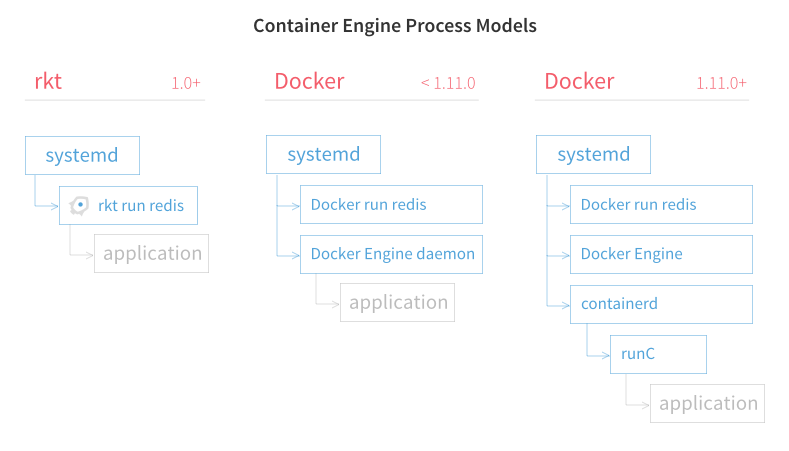
\includegraphics[scale=0.5]{img/rkt-vs-docker-process-model.png}
	\caption[Prozessmodelle im Vergleich zwischen rkt und Docker 
	\cite{rktvsdocker,}]{Prozessmodelle im Vergleich zwischen rkt und 
		\texttt{docker} \cite{rktvsdocker}}
	\label{fig:rkt_vs_docker}
\end{figure}
Wo bei \texttt{rkt} ein Prozess direkt gestartet wird, wird er bei 
\texttt{docker} über eine Engine verwaltet. Die direkte Verwaltung hat den 
Vorteil, dass es eine Abstraktionsschicht weniger gibt. Die Engine bietet 
dabei den Vorteil, dass man Containern die Möglichkeit gibt, sich selbst oder 
sogar andere Container in der Engine zu verwalten, ohne dass man dabei Zugriff 
auf das System geben muss. Die Abstraktionsebene kann also auch als 
Sicherheitslayer gesehen werden.

Ein Vergleich zwischen \texttt{docker} und \texttt{railcar} fällt schwer, da es 
keine wirklichen Unterschiede dazwischen gibt. Nach Aussage eines Entwicklers 
von \texttt{railcar} sind die Laufzeitkomponenten zu 98\% 
identisch.\cite{railcarvsdocker} Des Weiteren ist \texttt{railcar} nur ein 
drop-in für die Laufzeitkomponente von \ac{OCI} basierenden Applikationen.

Die Wahl zum Tool für die Prozessvirtualisierung fällt somit auf 
\texttt{docker}. Dieses Tool ist bereits seit einigen Jahren im Einsatz und 
hierzu gibt es bereits viele Lösungen und Dokumentationen durch die Community. 
Darüber hinaus ist \texttt{docker} bekannter, weswegen die Unterstützung 
bei \acf{IaaS} und \acf{PaaS} Anbietern einfacher ist.
\subsection{Orchestrierung} \label{subsec:tunorch}
Anders wie die Werkzeuge zur Prozessvirtualisierung, gibt es für die in Kapitel 
\ref{subsec:sdtorch} genannten Tools (\texttt{docker swarm}, \texttt{ansible}, 
\texttt{puppet} und \texttt{kubernetes}) keinen Standard. Schon beim 
Lesen der Webseiten der Produkte fällt auf, dass lediglich \texttt{kubernetes} 
direkt mit der Orchestrierung von Container-Engines wirbt.

In der aktuellen Lösung \cite{osmib} werden \texttt{ansibile}-Skripte 
eingesetzt, um die Container zu verwalten. Diese Lösung basiert auf 
einem einzelnen Container und müsste für die Orchestrierung stark erweitert 
werden. Die Mittel zur Container-Orchestrierung müssten hierbei selbst 
geschrieben werden, wie auch bei \texttt{puppet}.\cite{ansible}\cite{puppet}

\texttt{docker swarm} bietet keine direkte Möglichkeit, Orchestrierung zu 
betreiben. Anders wie \texttt{ansible} und \texttt{puppet}, ist
\texttt{docker swarm} direkt in \texttt{docker} integriert und 
kommuniziert somit nativ mit der Container-Engine. Auch hier müssten die 
Werkzeuge zur Orchestrierung selbst geschrieben werden.\cite{dockSwarm}

Unterschiedlich zu allen anderen genannten Werkzeugen bringt 
\texttt{kubernetes} sowohl alle Tools zur Verwaltung von Containern mit, als 
auch alles, um die Container zu orchestrieren. Es arbeitet eng mit der 
Container-Engine zusammen und es kann einfach von einem \texttt{docker swarm} 
dorthin migriert werden, sodass auch eine lokale Entwicklung leicht 
fällt.\cite{kubernetes}

Die Vorauswahl zum Tool für die Orchestrierung fällt somit auf
\texttt{docker swarm} oder \texttt{kubernetes}. Auch in der Community und 
Wirtschaft gibt es für diese Lösung eine breite Unterstützung und 
\texttt{kubernetes} ist der de-facto Standard für das Orchesteriren von 
Applikationen. Hier bieten schon viele \ac{PaaS}-Anbieter ein 
\glqq{}\texttt{kubernetes}-as-a-Service\grqq{} an. Es können sich allerdings 
auch andere Tools ergeben. Je nach Dienstleister oder vom Kunden gewünschten 
Verfahren können auch Technologien, wie z.B. CloudFoundry \cite{cloudfoundry} 
zum Einsatz kommen.
\clearpage
\subsection{Server und Umgebung}
\label{subsec:tunsu}
Die in Kapitel \ref{subsec:tunpv} beschriebenen Prozessvirtualisierungen 
eigenen sich für alle Linux basierten Systeme. Es werden nur freie 
Linuxdistributionen in Betracht gezogen, da die Firma, bei der diese Software 
entwickelt wird, ausschließlich freie Software entwickelt und auch nur freie 
Software verwendet. Es könnten auch BSD-Distributionen genutzt werden, jedoch 
fehlt die nötige Expertise, um sie in einem Event sicher einzusetzen. Andere 
Betriebssysteme, wie Windows oder Macintosh, können nicht genutzt werden, da 
sie nicht frei sind.

In Kapitel \ref{subsec:tunorch} wurde noch keine Entscheidung für die Software 
zur Orchestrierung gefällt. Die Wahl für das Werkzeug zur Orchestrierung wurde 
von der Bewertung für die Server und Umgebung abhängig gemacht. Zunächst wurden 
einige Anbieter für \ac{PaaS} und \ac{SaaS} angefragt. Diese Anbieter konnten 
meist alle mit \texttt{kubernetes} arbeiten, mindestens aber 
\texttt{docker-swarm} ausführen, oder haben es direkt angeboten. Bei der 
Besprechung mit den Anbietern ist aufgefallen, dass OpenSlides in kleineren 
Rahmen skaliert, als es für große Systeme, wie \texttt{kubernetes} nötig ist. 
Des Weiteren waren alle Anbieter so teuer, dass der Kostenfaktor in etwa um den 
Faktor 10 skalierte.

Die Wahl für die Server und Umgebung ist somit auf einen normalen Root-Server 
gefallen, mit der Nutzung von \texttt{docker-swarm} zur Orchestrierung. Mit 
diesem Aufbau kann die virtuelle Architektur zunächst aufgebaut und getestet 
werden. Der Aufbau bringt den Vorteil mit sich, dass die Migration von 
\texttt{docker-swarm} zu \texttt{kubernetes} gut beschrieben ist, und ein 
etablierter Pfad existiert. Es wird nicht direkt \texttt{kubernetes} verwendet, 
da der Mehraufwand, welcher durch die Komplexität von \texttt{kubernetes} 
entsteht, zu groß ist.
\clearpage
\section{Umsetzung - OpenSlides}
\label{sec:umsos}
Die Umsetzung erfolgt in mehreren Schritten. Zunächst wird OpenSlides in die 
einzelnen Container (\ref{subsec:umsoscont}) aufgeteilt; diese werden dann 
mittels \texttt{docker-compose} (\ref{subsec:umsoscom}) die Infrastruktur 
konfigurieren und diese wird mit Hilfe von \texttt{docker-swarm} 
(\ref{subsec:umsds}) gesteuert.

In Kapitel \ref{subsec:umsoscont} werden zunächst die erstellten 
Docker-Container erläutert, welche dann in Kapitel \ref{subsec:umsoscom} zum 
Einsatz kommen. Das darauf folgende Kapitel \ref{subsec:umsds} beschreibt den 
Einsatz in \texttt{docker-swarm}. 
\subsection{Docker-Container}
\label{subsec:umsoscont}
Die einzelnen Container wurden nach dem in Kapitel \ref{subsubsec:introfotb} 
beschriebenen Paket entwickelt. Für einige Teile konnten dabei schon vorhandene 
Pakete aus der Community genutzt werden; für andere mussten diese wiederum 
selbst entwickelt oder angepasst werden. Dabei wird in folgende Schritte 
unterteilt:
\begin{itemize}
	\item \texttt{core} (Kern von OpenSlides)
	\item \texttt{web} (\texttt{Daphne} zur Web-Darstellung)
	\item \texttt{postgres} (Datenbank)
	\item \texttt{redis} (Zwischenspeicher)
	\item \texttt{worker} (Anfragenverarbeitung)
	\item \texttt{nginx} (Webserver und Proxy für Daphne)
	\item \texttt{letsencrypt} (SSL-Zertifikatsverwaltung)
	\item \texttt{pg-slave} (Datenbank Backupsystem)
	\item \texttt{filesync} (Backupsystem für statische Dateien)
	\item \texttt{postfix} (Mail Versender)
\end{itemize}

Diese Übersicht wurde an Abbildung \ref{fig:ostechbesch} angelehnt. Die 
Kommunikation der einzelnen Komponenten entspricht der Abbildung. Das 
\texttt{core} Image ist jedoch kein aktiver Teil des Aufbaus, sondern erstellt 
lediglich statische Daten, auf die einzelne Komponenten zugreifen, und 
übernimmt die Erst-Konfiguration.
\newpage

\begin{figure}[htp]
	\centering
	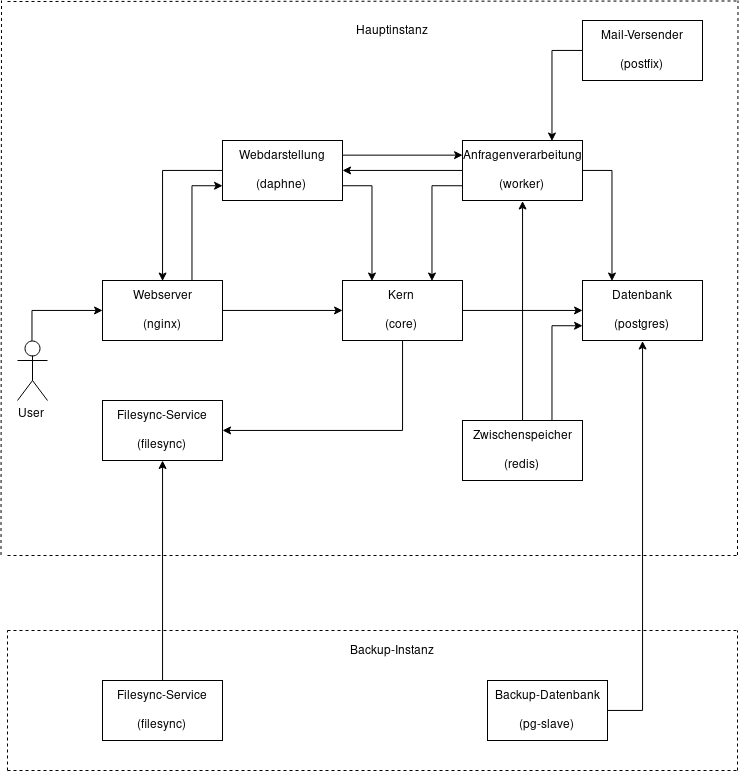
\includegraphics[width=0.87\textwidth]{img/dock_cont.png}
	\caption[OpenSlides - Docker Container Aufbau]{OpenSlides - Docker 
		Container Aufbau}
	\label{fig:osdockcont}
\end{figure}

Abbildung \ref{fig:osdockcont} beschreibt den Aufbau, den eine Instanz annehmen 
kann. Der \texttt{core} ist dabei kein aktiver Service, sondern stellt nur 
passiv die Daten für andere Services bereit. Ein User greift über seinen 
Browser auf den Webserver zu. Dieser leitet die Anfrage weiter zur 
Webdarstellung. Hier werden dynamisch hinterlegte Daten angefragt, die keiner 
weiteren Berechnung bedürfen. Statische Inhalte werden direkt vom Webserver 
ausgeliefert. Anfragen, die weiterer Berechnung bedürfen, werden an die 
Anfragenverarbeitung weitergeleitet, welche die Daten aus der Datenbank oder 
dem Zwischenspeicher lädt. Wenn die Anfrage verarbeitet wurde, wird sie wieder 
zurück über die Webdarstellung an den Webserver und schließlich in den Browser 
des Users geleitet.

Es kann eine Backup-Instanz eingerichtet werden, sodass über den 
Filesync-Service die statischen Daten getauscht werden können und ein Streaming 
mit einer Backup-Datenbank stattfindet. Wenn die erste Hauptinstanz ausfällt, 
kann der Filesync-Service und die Backup-Datenbank abgeschaltet werden, und alle 
anderen Services können gestartet werden, sodass man nach kurzer Zeit wieder 
ein intaktes System hat.

Der \texttt{core} konnte zu einem Teil aus dem offiziellen OpenSlides GitHub 
Reposity genommen werden \cite{osgh}. Um den Aufgaben zu entsprechen, musste er 
angepasst werden, sodass die Konfiguration dem Aufbau entspricht. Er richtet 
beim Start alle Komponenten ein und bei einem Upgrade führt er die 
entsprechenden Anpassungen in allen Konfigurationen durch und verteilt die 
neuen Daten.

Aus dem Dockerfile des OpenSlides GitHub Repositories wurde der Aufruf für den 
\texttt{Daphne} \cite{osgh} entnommen. Dieses Image erbt alle Eigenschaften des 
\texttt{core} Images, führt aber keine Anpassungen durch, sondern startet nur 
einen Service zur Web-Darstellung. Auf die gleiche Weise funktioniert auch das 
Image für den \texttt{worker}. Hier wird ein Prozess zur 
Anfragenverarbeitung gestartet.

Das Image für die \texttt{postgres}-Datenbank konnte aus der Community 
entnommen werden. Zunächst wurde das offizielle \texttt{postgres}-Image 
verwendet \cite{pgoffdock}. Dieses bietet leider nicht die Möglichkeit, den 
Datenstrom zu spiegeln, damit ein Backupsystem implementiert werden kann, 
weswegen die Version von \glqq{}sameersbn\grqq{} verwendet wird \cite{pgdock}.
Für das \texttt{redis}-Image wurde das offizielle Image verwendet 
\cite{reddock}.

Für den Webserver und die Zertifikatsverwaltung wurde eine Entwicklung aus der 
Community von \glqq{}jwilder\grqq{} und \glqq{}JrCs\grqq{} verwendet. Diese 
macht es möglich, dass gestartete Container zur Webdarstellung automatisch als 
Route aufgenommen werden \cite{nginxjwilderdock}. Das Image zur Verwaltung der 
Let's Encrypt basierten SSL-Zertifikate\cite{letsencrypt} arbeitet mit dem 
Image für \texttt{nginx} zusammen\cite{lejrcsdock}.

Um auch Mails zu versenden, wurde das \texttt{postfix}-Image von 
\grqq{}catatnight\glqq{} aus der Community verwendet\cite{postfixdock} und 
leicht angepasst, sodass es auf einem aktuellen Stand, ist und die 
Logging-Outputs an zentraler Stelle zusammen gefasst werden können.

Das \texttt{filesync}-Image wurde erstellt, damit Kunden Zugriff auf ihre 
statischen Daten für Backups haben und, um diese automatisch von 
einer zweiten Instanz spiegeln zu können. Dieses Image ist eine 
Eigenentwicklung.

Um auch ein Backup der Datenbank automatisch anlegen zu können, wurde vom 
gleichen Image, wie auch bei \texttt{postgres} das \texttt{pg-slave}-Image 
erstellt, welches die Daten aus einem anderen \texttt{postgres}-Image empfangen 
kann.
\newpage
\subsubsection{\texttt{core}, \texttt{web}, \texttt{worker}-Image}
Für das \texttt{core}-Image konnte das Docker Image aus dem offiziellen 
OpenSlides \cite{osgh} Repository zum Vorbild genommen werden. Es musste jedoch 
überarbeitet werden.
\begin{lstlisting}[firstnumber=1,
	caption=Dockerfile für den Bau des \texttt{core} - Teil 1 \cite{osdockcont},
	label={list:core1}]
from python:3.5

ARG BRANCH
ARG REPOSITORY_URL
ARG COMMIT_HASH

RUN mkdir /app

RUN apt-get update && \
	apt-get upgrade -y &&\
	apt-get install -y libpq-dev supervisor curl vim
RUN wget https://nodejs.org/dist/v6.11.3/node-v6.11.3-linux-x64.tar.xz -P /tmp
RUN cd /tmp && tar xfvJ node-v6.11.3-linux-x64.tar.xz
RUN ln -sf /tmp/node-v6.11.3-linux-x64/bin/node /usr/bin/node
RUN useradd -m openslides
RUN chown -R openslides /app
WORKDIR /app

USER openslides
RUN git clone -b $BRANCH $REPOSITORY_URL .
RUN git reset --hard $COMMIT_HASH
RUN rm -rf .git
\end{lstlisting}
Die Argumente in Listing \ref{list:core1} in Zeile 3-5 sind in Zeile 20 und 21 
dafür verantwortlich, dass eine spezifizierte Version gebaut werden kann. Unter 
\texttt{BRANCH} kann ein Branch eines Git-\texttt{REPOSITORY} angegeben werden. 
Aus diesem Branch kann dann der \texttt{COMMIT\_HASH} gebaut werden. Allerdings 
können nicht beliebige Versionen gebaut werden. Lediglich Versionen, die den 
gleichen Bauablauf und die gleichen Abhängigkeiten (vgl. Zeile 9-16 in Listing 
\ref{list:core1} und Zeile 23-33 in Listing \ref{list:core2}) haben.
\begin{lstlisting}[firstnumber=23,
	caption=Dockerfile für den Bau des \texttt{core} - Teil 2 \cite{osdockcont},
	label={list:core2}]
USER root
RUN pip install -r requirements_big_mode.txt
RUN rm -rf /var/lib/apt/lists/*

USER openslides
RUN curl -o- -L https://yarnpkg.com/install.sh | bash
RUN $HOME/.yarn/bin/yarn --non-interactive

RUN node_modules/.bin/gulp --production
RUN rm -fr bower_components
RUN rm -fr node_modules
\end{lstlisting}
\newpage
\begin{lstlisting}[firstnumber=34,
	caption=Dockerfile für den Bau des \texttt{core} - Teil 3 \cite{osdockcont},
	label={list:core3}]
USER openslides
RUN python manage.py createsettings
RUN sed -i 's/use_redis = False/use_redis= True/' personal_data/var/settings.py
RUN sed -i 's#redis://127.0.0.1:6379/0#redis://redis:6379/0#' personal_data/var/settings.py
RUN sed -i 's/EMAIL_HOST =/#EMAIL_HOST =/' personal_data/var/settings.py
RUN sed -i 's/EMAIL_PORT =/#EMAIL_PORT =/' personal_data/var/settings.py
RUN sed -i 's/EMAIL_HOST_USER =/#EMAIL_HOST_USER =/' personal_data/var/settings.py
RUN sed -i 's/EMAIL_HOST_PASSWORD =/#EMAIL_HOST_PASSWORD =/' personal_data/var/settings.py
RUN echo "\
CHANNEL_LAYERS['default']['CONFIG']['hosts'] = [('redis', 6379)]\
" >> personal_data/var/settings.py

RUN echo "\
SESSION_ENGINE = 'redis_sessions.session'\
" >> personal_data/var/settings.py
RUN echo "\
SESSION_REDIS_HOST = 'redis'\
" >> personal_data/var/settings.py
RUN echo "\
SESSION_REDIS_PORT = 6379\
" >> personal_data/var/settings.py
RUN echo "\
SESSION_REDIS_DB = 0\
" >> personal_data/var/settings.py

RUN echo "DATABASES = {\ 
	'default': {\
		'ENGINE': 'django.db.backends.postgresql',\
		'NAME': 'openslides',\
		'USER': 'openslides',\
		'PASSWORD': 'openslides',\
		'HOST': 'postgres',\
		'PORT': '5432',\
	}\
}\
\
" >> personal_data/var/settings.py
RUN echo "\
EMAIL_HOST = 'postfix'\
" >> personal_data/var/settings.py
RUN echo "\
EMAIL_PORT = 25\
" >> personal_data/var/settings.py
RUN echo "\
EMAIL_HOST_USER = 'openslides'\
" >> personal_data/var/settings.py
RUN echo "\
EMAIL_HOST_PASSWORD = 'openslides'\
" >> personal_data/var/settings.py
\end{lstlisting}
In Listing \ref{list:core3} werden die Einstellungen in die Einstellungs-Datei 
geschrieben, sodass sie in dem geteilten Aufbau funktionieren. Die Parameter 
werden in Kapitel \ref{subsec:umsoscom} erläutert. In Zeile 35 wird die 
Einstellungsdatei erstellt. In den beiden darauf folgenden Zeilen wird der 
\texttt{redis} konfiguriert. Zwischen Zeile 38 und 41 wird der Mailversand 
eingestellt und in Zeile 43 wird der \texttt{redis} dem \texttt{worker} bekannt 
gemacht. In den Zeilen 46-57 werden die Einstellungen mit dem \texttt{redis} 
eingestellt, ab Zeile 59 wird die Verbindung zum \texttt{postgres} beendet. 
Die Einstellungen zwischen Zeile 36 und 41 werden in der ursprünglichen 
Einstellung ersetzt. Die darauf folgenden Einstellungen werden an das Dokument 
angehangen, somit werden die Variablen überschreiben.

Diese Image-Beschreibungen wurden als \texttt{Dockerfile} gespeichert und 
können dann mit dem Befehl in Listing \ref{list:dockerbuild}
\begin{lstlisting}[numbers=none,
	caption=Befehl zum erzeugen eines Images,
	label={list:dockerbuild}]
docker build --tag tagname--build-arg argument=value
\end{lstlisting}
gebaut werden. Sobald das Image gebaut ist, liegt es in einer lokalen 
Image-Registry vor, und von dem Image können dann Container erzeugt werden. Die 
Container können über den Befehl in \ref{list:dockerrun} gestartet werden.
\begin{lstlisting}[numbers=none,
	caption=Befehl zum starten eines Containers,
	label={list:dockerrun}]
docker run -p interner-port:externer-port tagname
\end{lstlisting}
\texttt{}
Der \texttt{tagname} referenziert dabei auf das vorher erstellte 
Image.

Nimmt man das \texttt{Dockerfile} aus Listing \ref{list:core1} bis 
\ref{list:core3} von Zeile 1-35, so kann man eine einfache, nicht für 
produktive Einsätze geeignete, OpenSlides Version bereitstellen, welche die 
eingebaute Datenbank und Caching-Features nutzt. Dies wurde auch im ersten 
Schritt gemacht. Die Optionen nach Zeile 35 in Listing \ref{list:core3} sind 
mit den weiteren Images und deren Nutzung im Gesamtumfeld hinzu gekommen.

In Listing \ref{list:core3} kann man in Zeile 37 oder 43 sehen, dass als 
Hostname für den \texttt{redis} (analog Zeile 65 für \texttt{postgres} oder 
Zeile 72 für \texttt{postfix}) lediglich ein Service-Name angegeben wurde. Dies 
ist im Docker-Umfeld möglich, da die Docker Engine selbst einen DNS betreibt, 
der die Namen für die Services auflöst.
\begin{lstlisting}[firstnumber=1,
	caption=Dockerfile für den Bau des \texttt{web} - \cite{osdockcont},
	label={list:web}]
from openslides

CMD DJANGO_SETTINGS_MODULE=settings \
	PYTHONPATH=personal_data/var/ \
	daphne openslides.asgi:channel_layer -p 8000 -b 0.0.0.0 
\end{lstlisting}
Die erste Zeile im Listing \ref{list:web} zeigt die Vererbung von einem Image 
namens \texttt{openslides} an. Der in Kapitel \ref{subsec:umsoscom} erklärte 
Aufbau, baut das in Listing \ref{list:core1} bis \ref{list:core3} und nennt es 
\texttt{openslides}. Somit kann der \texttt{daphne} aus Listing \ref{list:web} 
und der \texttt{worker} aus \ref{list:worker} auf der gleichen Datengrundlage 
und mit dem gleichen Quellcode gestartet werden. Deswegen wird auch das Listing 
\ref{list:core1} bis \ref{list:core3} auch als \texttt{core} bezeichnet. Im 
Umkehrschluss bedeutet es auch, wenn ein neuer \texttt{core} eingesetzt werden 
soll, falls z.B. die Version verändert werden soll, müssen neben dem 
\texttt{core} Image auch das \texttt{web} und \texttt{worker}-Image neu gebaut 
werden.
\begin{lstlisting}[firstnumber=1,
	caption=Dockerfile für den Bau des \texttt{worker} - \cite{osdockcont},
	label={list:worker}]
from openslides

CMD sleep 5 && python manage.py runworker
	daphne openslides.asgi:channel_layer -p 8000 -b 0.0.0.0 
\end{lstlisting}
\newpage
\subsubsection{\texttt{filesync}-Image}
\begin{lstlisting}[firstnumber=1,
	caption=run.sh für das \texttt{filesync}-Image - \cite{osdockcont},
	label={list:fsyncrun}]
#!/bin/bash
shopt -s extglob 

sleep 25

while true
do
	if [ "$REMOTE_MODE" == "SLAVE" ]; then
		echo "Start backing up static files from https://$REMOTE_HOST"
		wget --quiet --http-password=$REMOTE_PASS --http-user=$REMOTE_USER -nH https://$REMOTE_HOST/static-backup/backup.zip
		echo "Done Downloading - Start copying"
		rm -rf static/*
		unzip backup.zip -d tmp
		mkdir -p static
		mkdir -p static/var
		mv tmp/static/var/* static/var
		rm -rf backup.zip
		rm -rf tmp
		chown openslides -R static
		echo "Backup Done - Sleeping for 5m"
	fi;
		if [ "$REMOTE_MODE" == "MASTER" ]; then
		echo "Start backing up static files"
		zip -r backup.zip static/var/*
		mkdir -p static/backup
		mv backup.zip static/backup
		echo "Backup Done - Sleeping for 5m"
	fi;
	sleep 600
done
\end{lstlisting}
In Listing \ref{list:fsyncrun} ist ein einfaches Skript, welches die statischen 
Dateien einer OpenSlides Instanz alle 5 Minuten in einen Ordner namens 
\texttt{static} verschiebt, oder eben jene Dateien von einer anderen Instanz 
aus in den \texttt{static} Ordner verschiebt. Dieses Script wird in dem Image, 
welches aus Listing \ref{list:fsdocker} gebaut wird, ausgeführt.
\begin{lstlisting}[firstnumber=1,
	caption=Dockerfile für den Bau des \texttt{filesync} - \cite{osdockcont},
	label={list:fsdocker}]
FROM debian:stretch

RUN mkdir /app

RUN apt-get update && \
apt-get upgrade -y &&\
apt-get install -y zip wget 

COPY run.sh /app/run.sh
RUN useradd -m openslides
WORKDIR /app

CMD ["/app/run.sh"]
\end{lstlisting}
\newpage
\subsubsection{\texttt{postfix}-Image}
Das Image für den Mailversand aus Listing \ref{list:postdock} erbt, wie in 
Kapitel \ref{subsec:umsoscont} erläutert, von \glqq{}catatnight\grqq{}s 
Entwicklung\cite{postfixdock}. Allerdings wird es zunächst in Zeile 3 bis 5 
geupdated und dann werden die Logging-Ausgaben in den allgemeinen 
\texttt{/dev/stdout} und \texttt{/dev/stderr} umgeleitet. Aus diesen Buffern 
setzt sich der allgemeine Docker-Log zusammen.
\begin{lstlisting}[firstnumber=1,
	caption=Dockerfile für den Bau des \texttt{postgres} - \cite{osdockcont},
	label={list:postdock}]
from catatnight/postfix

RUN apt-get update && \
	apt-get upgrade -y && \
	rm -rf /var/lib/apt/lists/*

RUN ln -sf /dev/stdout /var/log/mail.log && \
	ln -sf /dev/stderr /var/log/mail.err
\end{lstlisting}
\subsubsection{\texttt{nginx}-Image}
Das \texttt{nginx}-Image ist vollständig, wie in Kapitel \ref{subsec:umsoscont} 
beschrieben, aus der Community. Es wurden einige Einstellungen daran geändert, 
um den Anforderungen zu entsprechen. In Listing \ref{list:nginxcps} wird die 
\texttt{custom\_proxy\_settings.conf} geändert, um die maximale 
Upload-Dateigröße, die übertragen werden kann, von $\unit[10]{Mb}$ auf 
$\unit[100]{Mb}$ zu erhöhen.
\begin{lstlisting}[firstnumber=1,
	caption=\texttt{custom\_proxy\_settings.conf} für das \texttt{nginx}-Image - \cite{osdockcont},
	label={list:nginxcps}]
client_max_body_size 100M;
\end{lstlisting}
\newpage
\begin{lstlisting}[firstnumber=1,
	caption=\texttt{default\_location} für das \texttt{nginx}-Image - 
	\cite{osdockcont},
	label={list:nginxdl}]
location ~* ^/(?!ws|wss|webclient|core/servertime|core/version|users/whoami|users/login|users/logout|users/setpassword|motions/docxtemplate|agenda/docxtemplate|projector|real-projector|static|media|rest|nginx).*$ {
	rewrite ^.*$ /static/templates/index.html;
}
location ~* ^/projector.*$ {
	rewrite ^.*$ /static/templates/projector-container.html;
}
location ~* ^/real-projector.*$ {
	rewrite ^.*$ /static/templates/projector.html;
}
location ~* ^/webclient.*$ {
	rewrite ^/webclient/(site|projector).*$ /static/js/webclient-$1.js;
}
location /static {
	alias /app/static/var/collected-static;
}

location /nginx_status {
	stub_status;
	access_log off;
}

location /static-backup {
	alias /app/static/backup;
	autoindex on;
	auth_basic "Restricted Content";
	auth_basic_user_file /etc/nginx/.htpasswd;
}
\end{lstlisting}
In Listing \ref{list:nginxdl} wird die \texttt{default\_location} 
umgeschrieben. OpenSlides erzeugt einige statische Dateien, die in bestimmten 
Ordnern abgelegt werden. Diese Einstellungen sorgen dafür, dass sie bei 
entsprechenden Anfragen gefunden werden. Die Anfragen für die dynamischen 
Inhalte werden weiter an den \texttt{daphne} gegeben. Dadurch, dass der 
\texttt{daphne} keine großen Daten ausliefern muss, wird das System entlastet. 
Des Weiteren wird zwischen Zeile 17 und 20 der \texttt{nginx\_status} 
aktiviert, sodass man zur Laufzeit erkennen kann, wie viele Personen auf die 
Instanz zugreifen. Die darauf folgenden Zeilen ermöglichen es, dem 
\texttt{filesync}-Image Backup-Daten herunterzuladen, oder bereitzustellen. 
Weiter sieht man in Zeile 25 und 26, dass dieser Bereich durch die Datei aus 
Listing \ref{list:nginxht} passwortgeschützt ist. 
\begin{lstlisting}[firstnumber=1,
	caption=\texttt{htpasswd} für das \texttt{nginx}-Image - 
	\cite{osdockcont},
	label={list:nginxht}]
openslides:$apr1$ilfQt2m.$bJ0fT2aVP971CNWcHKQ1w.
\end{lstlisting}
\newpage
\begin{lstlisting}[firstnumber=1,
	caption=\texttt{nginx.conf} für das \texttt{nginx}-Image - 
	\cite{osdockcont},
	label={list:nginxconf}]
user  nginx;
worker_processes  auto;

error_log  /var/log/nginx/error.log warn;
pid        /var/run/nginx.pid;


events {
	worker_connections  16384;
}


http {
	include       /etc/nginx/mime.types;
	default_type  application/octet-stream;

	log_format  main  '$remote_addr - $remote_user [$time_local] "$request" '
	'$status $body_bytes_sent "$http_referer" '
	'"$http_user_agent" "$http_x_forwarded_for"';

	access_log  /var/log/nginx/access.log  main;

	sendfile        on;

	keepalive_timeout  65;

	include /etc/nginx/conf.d/*.conf;
}
daemon off;
\end{lstlisting}
Es musste eine eigene \texttt{nginx.conf} hinterlegt werden, da die 
ursprüngliche Konfiguration lediglich 100 Verbindungen gleichzeitig haben 
konnte. Diese wurden in Zeile 9 des Listings \ref{list:nginxconf} auf $16384$ 
angehoben.

Anders wie im \texttt{postfix}-Image musste hier nicht die allgemeine 
Log-Ausgabe auf die Linux-Standard-Buffer umgelenkt werden, da dieses Image die 
Einstellungen schon vorgenommen hat.

Die verbleibenden Images: \texttt{letsencrypt}, \texttt{pg-slave}, 
\texttt{postfix} und \texttt{redis} konnten ohne weitere Anpassungen auf 
Dateiebene verwendet werden.
\newpage
\subsubsection{Entwicklungsverlauf}
Zunächst wurde ein einzelnes Image gebaut, welches nur den \texttt{core}, 
\texttt{web} und \texttt{worker} enthielt. Da OpenSlides mit einer 
minimal-Datenbank paketiert ist, konnte hiermit zunächst ein erster Prototyp 
gebaut und eine grundsätzliche Richtung für den Bauprozess gelegt werden.

Anschließend wurde es in 2 Images aufgeteilt. Zunächst wurden \texttt{web} und 
\texttt{core} in einem Image und \texttt{worker} in einem anderen betrieben. 
Dazu wurde eine Verbindung zwischen den Images aufgebaut, sodass der 
\texttt{worker} die Daten aus dem \texttt{web} empfangen konnte und umgekehrt.

Im nächsten Schritt wurde zunächst das offizielle \texttt{postgres}-Image 
\cite{pgoffdock} verwendet, um das \texttt{postgres}-Image bereit zu stellen und das \texttt{redis}-Image wurde auch aufgesetzt. Sie wurden zunächst händisch in die jeweiligen Einstellungen eingetragen.

Um mehrere \texttt{web}-Prozesse starten zu können, wurde im letzten Schritt 
dieser Phase das \texttt{nginx}-Image hinzugebracht. Hier wurde auch zunächst 
das offizielle \texttt{nginx}-Image verwendet \cite{nginxdock}. In diesem wurde 
für jeden \texttt{web} Container, der gestartet wurde, die Konfiguration 
entsprechend angepasst.

Das \texttt{filesync} und das \texttt{pg-slave}-Image sind erst mit der 
Entwicklung der \texttt{docker-compose}-Konfiguration hinzugekommen.
\clearpage
\subsection{\texttt{docker-compose}}
\label{subsec:umsoscom}
Die in Kapitel \ref{subsec:umsoscont} beschriebenen Images können mit Hilfe von 
\texttt{docker-compose} in eine Architektur gebracht werden. Dabei können 
Verbindungen unter den Containern geknüpft werden. Sie können sich 
Dateigrundlagen teilen und in Netzwerke aufgeteilt werden. Für OpenSlides 
ergibt sich dabei die in Abbildung \ref{fig:dockercompose} aufgezeigte 
Architektur.
\begin{figure}[htp]
	\centering
	\begin{tikzpicture}[node distance = 2.25cm,
						scale=1,
						every node/.style={scale=1}]
		\node [draw] (postgres) {postgres};
		\node [draw, left of=postgres] (redis) {redis}; 
		\node [draw, above left of=postgres] (core) {core};
		\node [draw, left of=redis] (worker1) {worker\_1};
		\node [draw, below=0.5cm of worker1] (worker2) {worker\_2};
		\node [below=0.1cm of worker2] (worker3) {$\vdots$};
		\node [draw, above left of=worker1] (postfix) {postfix};
		\node [draw, left of=worker1] (web1) {web\_1};
		\node [draw, below=0.5cm of web1] (web2) {web\_2};
		\node [below=0.1cm of web2] (web3) {$\vdots$};
		\node [draw, left=4cm of web2] (nginx) {nginx};
		\node [draw, above of=nginx] (letsencrypt) {Let's Encrypt};
		\node [draw, below right=1cm and 4cm of nginx] (filesync) {filesync};
		\node [draw, right of=filesync] (pgslave) {pg-slave};
		\node [draw,
				inner sep=13mm,
				label=below:Network: back,
				fit=(filesync) (postgres) (core) (filesync) (web1)] {};
		\node[draw,
				inner sep=5mm,
				label=above:Network: front,
				fit=(letsencrypt) (nginx)] {};
		\path [->]
			(letsencrypt) edge [] (nginx)
			(nginx) edge [] (web1)
			(nginx) edge [] (web2)
			(web1) edge [] (worker1)
			(web1) edge [] (worker2)
			(web2) edge [] (worker1)
			(web2) edge [] (worker2)
			(postfix) edge [] (worker1)
			(worker1) edge [] (redis)
			(worker2) edge [] (redis)
			(redis) edge [] (postgres)
			(nginx) edge [] (filesync)
			(core) edge [] (postgres);
	\end{tikzpicture}
	\caption[Visualisierung des Instanzaufbaus mit \texttt{docker-compose}
		\cite{osdockcont}]
		{Visualisierung des Instanzaufbaus mit \texttt{docker-compose} 
		\cite{osdockcont}}
	\label{fig:dockercompose}
\end{figure}
Zunächst werden die logischen Festplatten (\texttt{voluemes}) und die Netzwerke 
in Listing \ref{list:dockc11} aufgeteilt. Dabei werden die logischen 
Festplatten einerseits dafür genutzt, Dateien dauerhaft zu speichern, 
andererseits, damit mehrere Container die gleiche Datengrundlage haben können.
\begin{lstlisting}[firstnumber=152,
	caption=\texttt{docker-compose.yml} Teil 11 - 
	\cite{osdockcont},
	label={list:dockc11}]
volumes:
	dbdata:
	staticfiles:
	certs:
	redisdata:
	nginx_vhost:
	nginx_html:
	nginx_conf:
	nginx_dhparam:
networks:
	front:
	back:
\end{lstlisting}
\newpage
\begin{lstlisting}[firstnumber=3,
	caption=\texttt{docker-compose.yml} Teil 1 - 
	\cite{osdockcont},
	label={list:dockc1}]
core:
	build:
		context: ./core
	args:
		# Change according to your details
		REPOSITORY_URL: https://github.com/OpenSlides/OpenSlides.git
		BRANCH: master
		COMMIT_HASH: 03b17837ed2c88692f1b99ec5b9b477f86fdddb6
	image: openslides
	command: bash -c "rm -rf /app/personal_data/var/static && rm -rf /app/personal_data/var/collected-static && sleep 15 && python manage.py migrate && python manage.py collectstatic --noinput"
	depends_on:
		- postgres
	volumes:
		- "staticfiles:/app/personal_data"
	networks:
		- back
\end{lstlisting}
In Listing \ref{list:dockc1} wird der \texttt{core} Service zusammen gestellt. 
Hier werden die in \ref{list:core1} erwähnten Argumente und der Image-Name 
gesetzt. Im \texttt{command}-Block werden zunächst die vorhandenen 
Dateien entfernt und dann erneut erstellt. Bevor die Datenbank migriert werden 
kann, muss noch einige Zeit gewartet werden, um sicher zu stellen, dass der 
\texttt{postgres}-Service bereits gestartet ist. Die statischen Dateien werden 
dann im \texttt{staticfiles}-Volume gespeichert. Nachdem der Befehl 
abgeschlossen ist, schaltet sich der Service wieder ab.
\begin{lstlisting}[firstnumber=19,
	caption=\texttt{docker-compose.yml} Teil 2 - 
	\cite{osdockcont},
	label={list:dockc2}]
web:
	build: ./web
	image: os-web
	restart: always
	links:
		- redis
	depends_on:
		- core
		- nginx
	expose:
		- 8000
	environment:
		# Change according to your details
		VIRTUAL_HOST: 'localhost'
		LETSENCRYPT_HOST: 'localhost'
		LETSENCRYPT_EMAIL: 'localhost'
		LETSENCRYPT_TEST: 'true'
	volumes:
		- "staticfiles:/app/personal_data"
	networks:
		- back
\end{lstlisting}
Das Listing \ref{list:dockc2} baut den \texttt{web}-Service auf. Dieser wird 
mit dem \texttt{redis}-Service verbunden. Die Angaben im 
\texttt{environment}-Block machen dem \texttt{nginx}- und 
\texttt{letsencrpyt}-Service klar, dass dieser Service ansprechbar sein soll 
und unter welcher URL dieser erreicht werden muss. Auch dieser Service hat 
Zugriff auf die \texttt{staticfiles}.
\newpage
\begin{lstlisting}[firstnumber=40,
	caption=\texttt{docker-compose.yml} Teil 3 - 
	\cite{osdockcont},
	label={list:dockc3}]
redis:
	image: redis:alpine
	restart: always
	volumes:
		- "redisdata:/data"
	networks:
		- back
\end{lstlisting}
Der \texttt{redis}-Service in Listing \ref{list:dockc3} hat keine Möglichkeit, 
Daten dauerhaft zu speichern, da er lediglich ein Zwischenspeicher ist.
\begin{lstlisting}[firstnumber=47,
	caption=\texttt{docker-compose.yml} Teil 4 - 
	\cite{osdockcont},
	label={list:dockc4}]
worker:
	build: ./worker
	image: os-worker
	links:
		- redis
	depends_on:
		- core
	volumes:
		- "staticfiles:/app/personal_data"
	networks:
		- back
\end{lstlisting}
Das Listing \ref{list:dockc4} zum \texttt{worker}-Service basiert ebenfalls auf 
der Datengrundlage der \texttt{staticfiles}. Er kommuniziert, anders als 
der \texttt{web}-Service, nur mit dem \texttt{redis}-Service.
\begin{lstlisting}[firstnumber=58,
	caption=\texttt{docker-compose.yml} Teil 5 - 
	\cite{osdockcont},
	label={list:dockc5}]
nginx:
	image: jwilder/nginx-proxy
	restart: always
	volumes:
		- "/var/run/docker.sock:/tmp/docker.sock:ro"
		- "certs:/etc/nginx/certs:ro"
		- "nginx_vhost:/etc/nginx/vhost.d"
		- "nginx_html:/usr/share/nginx/html"
		- "nginx_conf:/etc/nginx/conf.d"
		- "nginx_dhparam:/etc/nginx/dhparam"
		- "staticfiles:/app/static:ro"
		- "./nginx/default_location:/etc/nginx/vhost.d/default_location"
		- "./nginx/htpasswd:/etc/nginx/.htpasswd"
		- "./nginx/custom_proxy_settings.conf:/etc/nginx/conf.d/custom_proxy_settings.conf"
		- "./nginx/nginx.conf:/etc/nginx/nginx.conf"
	ports:
	- "80:80"
	- "443:443"
	environment:
		- ENABLE_IPV6=true
	labels:
		com.github.jrcs.letsencrypt_nginx_proxy_companion.nginx_proxy: "true"
	networks:
		- front
		- back
\end{lstlisting}
Der \texttt{nginx}-Service in Listing \ref{list:dockc5} benötigt mehrere 
volumes, die er sich zum Teil mit dem \texttt{letsencrypt}-Service (Listing 
\ref{list:dockc6}) teilt. Der \texttt{nginx}-Service braucht, um Daten über 
eine \texttt{https} verschlüsselt bereit zu stellen, die Daten, die der 
\texttt{letsencrpt}-Service bereit stellt. Das \texttt{label} dient dem 
\texttt{letsencrpyt}-Service dazu, den \texttt{nginx}-Service zu 
identifizieren. Allerdings kann auch ein eigenes Zertifikat in den Ordner 
gelegt werden, falls ein automatisches Erstellen über \texttt{letsencrypt} 
nicht gewünscht ist. Damit der \texttt{nginx}-Service automatisch neue 
Instanzen des \texttt{web}-Service finden kann, braucht dieser einen Zugriff 
auf den \texttt{docker} Unix-Socket.
\begin{lstlisting}[firstnumber=83,
	caption=\texttt{docker-compose.yml} Teil 6 - 
	\cite{osdockcont},
	label={list:dockc6}]
letsencrypt:
	image: jrcs/letsencrypt-nginx-proxy-companion
	restart: always
	volumes:
		- "/var/run/docker.sock:/var/run/docker.sock:ro"
		- "certs:/etc/nginx/certs:rw"
		- "nginx_vhost:/etc/nginx/vhost.d"
		- "nginx_html:/usr/share/nginx/html"
		- "nginx_conf:/etc/nginx/conf.d"
	depends_on:
		- nginx
	environment:
		NGINX_PROXY_CONTAINER: nginx
	networks:
		- back
\end{lstlisting}
\begin{lstlisting}[firstnumber=98,
	caption=\texttt{docker-compose.yml} Teil 7 - 
	\cite{osdockcont},
	label={list:dockc7}]
postgres:
	image: sameersbn/postgresql:9.6-2
	restart: always
	volumes:
		- "dbdata:/var/lib/postgresql"
	environment:
		- DB_USER=openslides
		- DB_PASS=openslides
		- DB_NAME=openslides
		- REPLICATION_USER=repluser
		- REPLICATION_PASS=repluserpass
	ports:
		- "5432:5432"
	networks:
		- front
		- back
\end{lstlisting}
Die \texttt{postgres} und \texttt{pg-slave} Listings (\ref{list:dockc6} und 
\ref{list:dockc7}) speichern beide permanent in einem Ordner. Der 
\texttt{postgres}-Service ist dabei, eine normale Datenbank, und der 
\texttt{pg-slave}-Service kann von einer Datenbank, wie der im 
\texttt{postgres}-Service, die Daten streamen. Dadurch, dass beide Services in 
dem gleichen \texttt{volume} speichern, können sie untereinander ausgetauscht 
werden. Sie dürfen aber nie zur gleichen Zeit laufen.
\begin{lstlisting}[firstnumber=114,
	caption=\texttt{docker-compose.yml} Teil 8 - 
	\cite{osdockcont},
	label={list:dockc8}]
pg-slave:
	image: sameersbn/postgresql:9.6-2
	restart: always
	volumes:
		- "dbdata:/var/lib/postgresql"
	environment:
		- REPLICATION_MODE=slave
		- REPLICATION_SSLMODE=prefer
		- REPLICATION_HOST=127.0.0.1
		- REPLICATION_PORT=5432
		- REPLICATION_USER=repluser
		- REPLICATION_PASS=repluserpass
	networks:
		- back
\end{lstlisting}
\begin{lstlisting}[firstnumber=128,
	caption=\texttt{docker-compose.yml} Teil 9 - 
	\cite{osdockcont},
	label={list:dockc9}]
filesync:
	build: ./filesync
	image: os-filesync
	restart: always
	volumes:
		- "staticfiles:/app/static"
	environment:
		- REMOTE_MODE=MASTER
		- REMOTE_HOST=localhost
		- REMOTE_USER=openslides
		- REMOTE_PASS=openslides
	networks:
		- back
\end{lstlisting}
In Listing \ref{list:dockc9} wird der \texttt{filesync}-Service definiert. Hier 
wird im \texttt{environment}-Block festgelegt, ob er die Rolle des 
\texttt{MASTER} oder \texttt{SLAVE} (vgl. Listing \ref{list:fsyncrun}) 
übernimmt. Hier werden auch die Nutzerdaten aus dem Listing \ref{list:nginxht} 
eingetragen. Er bekommt Zugriff auf die \texttt{staticfiles}, sodass der 
\texttt{nginx}-Service diese ausliefern kann.
\begin{lstlisting}[firstnumber=141,
	caption=\texttt{docker-compose.yml} Teil 10 - 
	\cite{osdockcont},
	label={list:dockc10}]
postfix:
	build: ./postfix
	image: postfix
	restart: always
	environment:
		- maildomain=localhost 
		- smtp_user=openslides:openslides
	volumes:
		- "certs:/etc/postfix/certs:ro"
	networks:
		- back
\end{lstlisting}
Der \texttt{postfix}-Service in Listing \ref{list:dockc10} hat lediglich 
Zugriff auf die Zertifikate, damit dieser verbindungsverschlüsselt versenden 
kann. Die Variablen im \texttt{environment} werden benötigt, um den Service in 
OpenSlides korrekt konfigurieren zu können.
\subsubsection{Entwicklungsverlauf}
Zunächst wurde der \texttt{core} Service aufgesetzt, wie im vorherigen Kapitel 
beschrieben, in der kleineren Version im Listing \ref{list:core1} bis 
\ref{list:core3} von Zeile 1-35.

Danach wurde der \texttt{postgres} hinzugefügt und ein Teil der 
Einstellungsänderung aus Listing \ref{list:core3} hinzugefügt. Nachdem die 
Verbindung zwischen den beiden erfolgreich hergestellt werden konnte, wurde der 
\texttt{redis} angefügt. Danach konnte der \texttt{web} und \texttt{worker} aus 
dem \texttt{core} heraus gelöst und als eigener Service angesetzt werden.

Anschließend wurde der \texttt{nginx} und \texttt{letsencrpyt} mit dem 
\texttt{postgres} Service hinzugefügt, damit eine verschlüsselte Verbindung 
aufgebaut werden konnte.

Schlussendlich wurden die \texttt{pg-slave} und \texttt{filesnyc}-Images 
aufgebaut und angefügt.
\clearpage
\subsection{\texttt{docker-swarm}}
\label{subsec:umsds}
Mit der in Kapitel \ref{subsec:umsoscom} erstellen Konfiguration für 
\texttt{docker compose} kann nun ein \texttt{stack} für \texttt{docker-swarm} 
gebaut werden. Ein Stack besteht aus einer Konfigurationsdatei von 
\texttt{docker compose}. Ein Stack kann in einem \texttt{swarm} deployed 
werden. Der \texttt{swarm} kann aus mehreren Servern bestehen, die 
einzelnen Images erzeugen und innerhalb des Schwarms verteilen. Last kann 
somit gleichmäßig verteilt werden. Es können auch mehrere \texttt{stacks} bzw. 
OpenSlides Instanzen in einem \texttt{swarm} gestartet werden.

In der Arbeit wurde eine Schwarm-Umgebung, bestehend aus mehr als einem Server 
im Schwarm vernachlässigt. Um mehrere Server in der Schwarm-Umgebung zu 
betreiben, müssen alle Server des Schwarms die Images kennen, dazu muss ein 
Registry-Server in der Umgebung registriert werden. Auf dieser Registry können 
die Images veröffentlicht werden und die Teilnehmer des Schwarms laden die 
Images von diesem Server herunter. Damit die Registry in der Umgebung 
funktionieren kann, muss sie mit TLS-Zertifikaten ausgestattet werden. Ohne 
diese können die Images nicht von den anderen Servern im Schwarm herunter 
geladen werden.

Es ergibt sich eine 
Architektur, die in Abbildung \ref{fig:dockerswarm} zu sehen ist.
\begin{figure}[htp]
	\centering
	\begin{tikzpicture}[node distance = 3cm,
						scale=1,
						every node/.style={scale=1}]
		\node [draw] (nginx) {nginx};
		\node [draw, right of=nginx] (registry) {registry};
		\node [draw, above=0.2cm of registry] (frontend) {frontend};
		\node [draw, above=0.2cm of frontend] (backend) {backend};
		\node [draw, above=0.2cm of backend] (portainer) {portainer};
		\node [draw, below right=0.8cm and 1.5cm of frontend]
			(OS1) {OpenSlides 1};
		\node [draw, below=0.5cm of OS1] (OS2) {OpenSlides 2};
		\node [draw, below=0.5cm of OS2] (OS3) {OpenSlides 3};
		\node [below=0.1cm of OS3] (OS4) {\vdots};
	
		\node[draw,
				inner sep=4mm,
				label=above:Network: back,
				fit=(portainer) (registry)] {};
		\node[draw,
				inner sep=2mm,
				label=left:Network: front,
				fit=(nginx)] {};
		\node[draw,
				inner sep=2mm,
				label=right:Network: OS1,
				fit=(OS1)] {};
		\node[draw,
				inner sep=2mm,
				label=right:Network: OS2,
				fit=(OS2)] {};
		\node[draw,
				inner sep=2mm,
				label=right:Network: OS2,
				fit=(OS3)] {};
		\path [->]
			(nginx) edge [] (portainer)
			(nginx) edge [] (backend)
			(nginx) edge [] (frontend)
			(nginx) edge [] (registry)
			(nginx) edge [bend right=35] (OS1)
			(nginx) edge [bend right=30] (OS2)
			(nginx) edge [bend right=25] (OS3);
	\end{tikzpicture}
	\caption[Visualisierung des Orchestrierungsaufbaus mit \texttt{docker-swarm}
		\cite{osman}]
		{Visualisierung des Instanzaufbaus mit \texttt{docker-compose}
		\cite{osman}}
	\label{fig:dockerswarm}
\end{figure}
Dadurch, dass \texttt{docker-swarm} auch auf mehreren Servern verteilt laufen 
kann, wird ein anderer \texttt{nginx} für das routing benötigt. Dieser hat auch 
Zugriff auf den Unix Sockel von Docker, er schaut jedoch danach, ob neue Stacks 
von OpenSlides gestartet werden und routet diese nach den Parametern aus der 
\texttt{docker-compose} Konfigurationsdatei.

Der \texttt{portainer} ist eine fertige Software, die bei der Überwachung und 
Übersicht über die Instanzen, auf der technischen Seite hilft. Hier werden die 
Log-Details der einzelnen Stacks zusammen gefasst, und man gewinnt eine 
Übersicht über den Status der einzelnen Instanzen.

Schlussendlich sind \texttt{backend} und \texttt{frontend} die Manager, welche 
die Konsolen-Operationen für Nutzer zur Verfügung stellen.

Da in den einzelnen OpenSlides Instanzen ein \texttt{nginx}-Image verwendet 
wird, welches den lokalen Docker-Socket nutzt und neue \texttt{web} Instanzen 
als Route aufnimmt, muss bei den Instanzen darauf geachtet werden, dass sie 
jeweils nur auf einem Server gestartet werden.

Um neue Instanzen bzw \texttt{stacks} in das Routing mit aufzunehmen, muss der 
\texttt{nginx} des Manageres zum deployen jedes neuen Stacks angepasst werden. 
Diese Funktionalität wird vom \texttt{backend} übernommen.
\subsection{Umsetzung - Multiinstance-Manager}
\label{sec:umm}
Im \texttt{backend} des Multiinstance-Managers werden letztendlich nur die 
Konsolenbefehle unter unterschiedlichen URLs mit  verschiedenen Parametern 
bereitgestellt. Diese können durch das Frontend angesteuert werden. Das 
\texttt{frontend} verarbeitet und visualisiert die Antworten.

In Kapitel \ref{subsec:ummb} wird die Funktion des \texttt{backend} erörtert. 
Das darauf folgende Kapitel \ref{subsec:ummf} beschreibt das \texttt{frontend}.
\subsubsection{\texttt{backend}} \label{subsec:ummb}
Zunächst werden die einzelnen Befehle und Schritte, die nötig sind, um eine neue Instanz zu starten und einzurichten, händisch durchgeführt. Diese wurden in einer \texttt{flask}-basierten \texttt{python}-Applikation in technisch 
zusammengehörigen Routen zusammengefasst.

Da das \texttt{backend} nur durch die Images im \texttt{back}-Network 
erreichbar ist und nur durch das \texttt{frontend} ansteuerbar ist, werden 
keine zusätzlichen Absicherungen für Aufrufe benötigt. Die Routen im 
\texttt{backend} sind nur aufrufbar, wenn das \texttt{frontend} übernommen wird,
oder eine Angreiferin sich Zugriff auf den Server verschafft.
\subsubsection{\texttt{frontend}} \label{subsec:ummf}
Das \texttt{frontend} bietet Zugriff auf die im \texttt{backend} erstellten 
Funktionen, um die Instanzen zu steuern oder koordinieren. Es basiert auf einer 
\texttt{django}-Applikation, um die Nutzer und die Zugehörigkeit dieser zu den 
einzelnen Instanzen, so wie deren Berechtigungen zu verwalten.

Zugriff auf das \texttt{frontend} ist nur für Personen nötig, welche die 
Instanzen technisch betreuen müssen. Hier wird darauf geachtet, dass die 
einzelnen Instanzen auch nur von den Nutzern verwaltet werden können, die die 
entsprechenden Rechte haben.
\clearpage
\section{Zusammenfassung und Ausblick}
\label{sec:za}
In Kapitel \ref{subsec:zaze} werden die Ergebnisse dieser Arbeit zusammen 
gefasst und in Kapitel \ref{subsec:zaa} wird ein Ausblick auf kommende 
Entwicklungen gegeben.
\subsection{Zusammenfassung der Ergebnisse} \label{subsec:zaze}
In dieser Arbeit wurde die Virtualisierung von OpenSlides in Ausblick auf einen 
Multiinstanz-Kontext auf der Basis von Docker entwickelt. Des Weiteren wurde 
ein Proof of Concept für den Multiinstanz-Betrieb erstellt.

Die Entwicklungen dieser Arbeit wurden auf GitHub unter
\url{http://github.com/OpenSlides/openslides-docker} und
\url{https://github.com/jsaalfeld/openslides-manager} bereit gestellt. Weitere 
kleinere Arbeiten wurden an OpenSlides direkt durchgeführt 
(\url{http://github.com/OpenSlides/OpenSlides}).

Zunächst wurde eine Einführung in das Thema gegeben und die 
Versammlungssoftware OpenSlides wurde erklärt. Anschließend wurden verschiedene 
Tools zur Prozessvirtualisierung und Orchestrierung erörtert und es wurde 
erklärt, welche Tools für die Umsetzungen verwendet werden. Darauf hin wurde die 
Umsetzung beschrieben.

Die bisherige Virtualisierung von OpenSlides war bislang nur in einem 
nicht-skalierbaren Modus möglich und basierte auf \texttt{rkt}. Diese wurde 
durch \texttt{docker} abgelöst und die Software-Architektur wurde auf neuere 
Versionen angepasst und für einen produktiven Einsatz in einem großen Umfeld 
umgesetzt.

Dadurch, dass die einzelnen Komponenten getrennt von einander laufen, und die 
Software eine einfache Aktualisierung unterstützt, ist der administrative 
Aufwand sehr gering, und die Kosten für den eigenen Server sind auch günstig. 
Somit konnte das allgemeine Ziel der Kostenreduktion erreicht werden. In 
Zukunft könnte hier noch besser geplant werden, wenn Kunden nicht nur 
Mietzeiträume angeben, sondern auch den eigentlich Durchführungszeitraum der 
Veranstaltung. So könnte genau geplant werden, wann und ob große Veranstaltungen
zusammen fallen, sodass zusätzliche Hardware kurzfristig dazu oder 
abgeschaltet werden kann.

Die Grundstruktur des \texttt{docker-compose} Aufbaus, welches in Kapitel 
\ref{subsec:umsoscom} beschrieben wurde, war bereits erfolgreich beim 
DGB-Bundeskongress 2018 in Berlin im Einsatz\cite{dbgbuko}. Bei vorherigen 
Veransaltungen vom DGB, wie dem Bundesjugendkonferenz\cite{dgbjuko} des DGB, 
wurde der alte Multiinstance-Server eingesetzt. Durch die Dynamik der 
Neuentwicklungen konnte einfacher auf plötzlich steigende Anfragen reagiert 
werden, und der Einsatz verlief reibungslos.

Die Entwicklungen des Multiinstance-Backend hat in einem großen Teil das 
bisherige Backend abgelöst. Diese Entwicklungen und bisherigen Erkenntnisse 
werden den anderen OpenSlides Entwicklern vorgestellt, um das weitere Vorgehen 
zu besprechen.
\newpage
\subsection{Ausblick} \label{subsec:zaa}
Die Lösung soll wartungsärmer werden und sowohl bei größeren Kunden zum Einsatz 
kommen als auch eine Zentralinstanz zum Anbieten von Einzelinstanzen aufgesetzt 
werden. Somit können Kunden günstige Einzelinstanzen angeboten werden. Hier 
soll auch ein automatisches Bezahlsystem implementiert werden, sodass die 
Instanzen so lange aktiv sind, wie für sie bezahlt wird.

Weitere Ideen für Weiterentwicklungen umfassen:
\begin{itemize}
	\item Anbindung von Identitäsverwaltungen
	\item Single-Sign-On über mehrere Instanzen
	\item Automatisches, georedundantes Backup
	\item Zentrale Übersicht und Fehlersammelstelle
	\item Softwaregestützte Upgrademechanismen
\end{itemize} 
\clearpage
\section*{Akronyme}
\begin{acronym}[Bash]
	\acro{IaaS}{Infrastructure as a Service}
	\acro{PaaS}{Platform as a Service}
	\acro{SaaS}{Software as a Service}
	\acro{OCI}{Open Container Initiative}
	\acro{OSMIB}{OpenSlides Multiinstace Backend}
	\acro{PPU}{Pay per use}
\end{acronym}
\clearpage
\bibliographystyle{./plaindin}
\bibliography{biblist.bib}
%\clearpage
%\appendix
%\section*{Docker-Umgebung}
%\begin{lstlisting}
%version: '3'
%...
%\end{lstlisting}
%\addappheadtotoc
\clearpage
\section*{Erklärung zur selbstständigen Abfassung der Bachelorarbeit}
Ich versichere, dass ich die eingereichte Bachelorarbeit selbstständig und ohne 
unerlaubte Hilfe verfasst habe. Anderer, als der von mir angegebenen 
Hilfsmittel und Schriften, habe ich mich nicht bedient. Alle wörtlich oder 
sinngemäß der Schriften anderer entnommenen Stellen habe ich kenntlich gemacht.

\vspace{8em}

\dots\dots\dots\dots\dots\dots\dots\dots\dots\dots\dots\dots\dots\dots\dots
\dots\dots\dots\dots\dots\dots\dots\dots\dots\dots\dots\dots\dots\dots\dots

Ort, Datum, Unterschrift
\end{document}